In this chapter, we throughly describe the Time Stamped Tries approach
to implement a subsumptive tabling engine. This mechanism was proposed by
Ernie Johnson \textit{et al}. \cite{Johnson-99} and is currently implemented in XSB.
It is based on the idea of extending each answer trie node with \textit{time stamp}
information as a means to distinguish between new answers and old answers.

First, we start by describing the algorithms and data structures associated
with the detection of subsuming goals. Next, we explain the data structures
introduced in the answer tries to support subsumption, focusing on answer insertion
and retrieval for subsumed subgoals. Finally, we describe the modifications made to the YapTab
tabling engine in order to support subsumptive tabling, focusing on the tabling operations
and on the table space.

\section{Finding General Subgoals}\label{sec:lookup_subsuming}

The problem of finding on a subgoal trie $C$ a subgoal $G'$ that subsumes $G$ 
is an important part of a subsumptive tabling engine, as it makes possible to
identify a subsumptive relation between $G'$ and $G$.

In the SLG-WAM, the search is performed by recursively backtracking through the subgoal trie $C$, trying
to match the node symbols with sub-terms from $G$. The process stops once a leaf node is reached.

The matching process gives priority to match non-variable terms from $G$
with an identical symbol from $C$.
Alternatively, if the current trie symbol is a variable, for example \texttt{VAR0}, on its first occurrence, \texttt{VAR0}
is bound to the respective $G$ sub-term
and match succeeds. On the next occurrences, the current sub-term from $G$ must
be identical to the term bound to \texttt{VAR0}. Throughout the search process, bound variables are
matched before new unbound variables.

Favoring non-variable terms, results in a mechanism that finds \textit{minimally subsuming calls}.
In particular, if there is a variant trie path of $G$ called $G''$, $G''$ is found before any other subgoal.
If no variant path exits, it is possible to speedup the process of inserting a variant path of $G$
by recording the trie node where: (1) the first constant match
failure occurred; or (2) an already seen $G$ variable paired to a trie variable could
not be paired to the same trie variable.

\begin{figure}[ht]
  \centering
    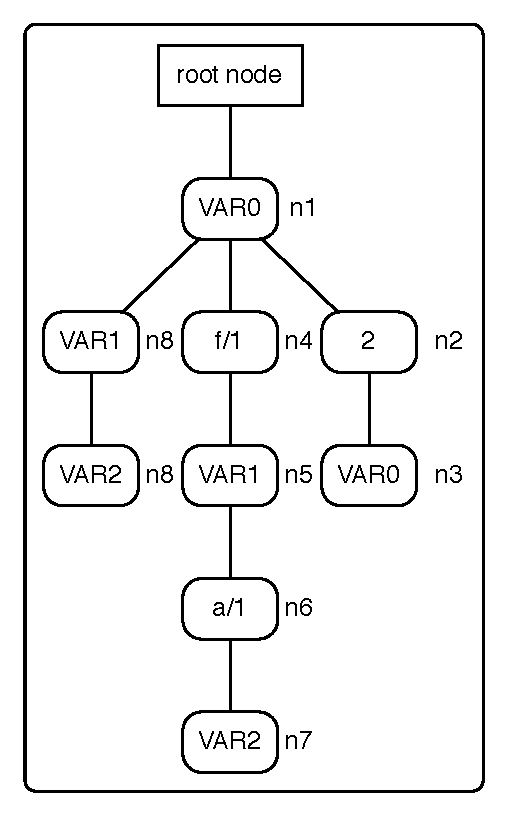
\includegraphics[scale=0.6]{sub_call_search.pdf}
  \caption{Subgoal trie for a tabled predicate \texttt{p/3}.}
  \label{fig:sub_call_search}
\end{figure}

For illustration purposes, Figure~\ref{fig:sub_call_search} shows a subgoal trie for a tabled predicate \texttt{p/3}.
The first subgoal called was \texttt{p(X,2,X)}, followed by \texttt{p(X,f(Y),a(Z))} and finally \texttt{p(X,Y,Z)}.

If the subgoal \texttt{p(X,2,X)} is called again, the algorithm described above
should find the variant subgoal represented by the leaf node $n3$. First, we unify the trie variable
\texttt{VAR0} with \texttt{X} (node $n1$), hence we must mark the variable \texttt{X} as \textit{seen},
because if the same variable appears again it must unify with the same trie variable for a variant path
to exist. Next, \texttt{2} easily unifies with trie node $n2$ and unification proceeds. In trie node $n3$,
the current call term is \texttt{X} and we also have a variable in the trie node. As \texttt{X} was already seen before,
it must unify with \texttt{VAR0}. It does and thus a variant path is found. Please note that if
the trie symbol at node $n3$ was \texttt{VAR1} no variant path would exist, but the process could proceed
and a subsuming subgoal would be found, as \texttt{p(VAR0,2,VAR1)} subsumes \texttt{path(VAR0,2,VAR0)}.
In this case, a variant path could be created by resuming the insert operation at node $n2$ to insert
a \texttt{VAR0} node.

For a more complex example, let the subgoal \texttt{p(2,f(X),a(2))} now be called for the same subgoal trie. First,
the algorithm searches for a trie node with the symbol \texttt{2}, and as it does not find one, no variant path
exists in this subgoal trie. Next, the algorithm tries to unify with bound variables, but as the process
has just started, only unbound variables are found, and \texttt{VAR0} (node $n1$) is unified with \texttt{2}.
The functor term \texttt{f/1} is the next term on the subgoal and node $n4$ matches with it.
The next term is \texttt{X} and it can unify with \texttt{VAR1} (node $n5$).
Note that if we failed at this point, the process would backtrack to node $n1$ and node $n8$
would be tried next, which would lead to a more general subgoal.
Next, the functor term \texttt{a/1} matches with trie node $n6$ and the process proceeds.
The last term symbol \texttt{2} can match with node $n7$, as it is an unbound variable
and the only node available.
If the variable was bound, like \texttt{VAR0} for instance,
the process would check if the current term symbol unifies with the variable binding made before (\texttt{VAR0=2}) and
it would also succeed. As node $n7$ is a leaf node, the process finishes with a subsumptive path found and
the following variable bindings made: \texttt{VAR0=2}, \texttt{VAR1=X}, and \texttt{VAR2=2}.

Implementation wise, this algorithm uses the following data structures:

\begin{itemize}
  \item \textit{variable bindings vector}: saves bindings for each numbered trie variable. Starts with each position pointing to itself;
  \item \textit{variable enumerator vector}: when a never seen term variable appears it must be bound to a position in this enumerator, ensuring that it can be recognized if the same variable appears a second time;
  \item \textit{term stack}: stores the remaining terms to be unified against the trie symbols;
  \item \textit{term log stack}: stores already matched terms taken from the term stack. Each frame contains the top index and the top element of the term stack during the creation of a frame;
  \item \textit{trail stack}: stores bindings that were made during the process. It is used to untrail variables during backtracking;
  \item \textit{call choice point stack}: used to restore the search process at a certain node to explore alternatives.
\end{itemize}

During execution, two matching methods are considered: the first tries to match exact trie symbols against the current term;
the second method uses trie variables instead of exact symbols and is employed when the first method fails.
When a trie node match succeeds, matching defaults to the first method, which means
that exact matches are always tried before variables when a new \textit{trie level} is reached and variables are usually attempted
when backtracking. A trie level represents a set of nodes that are linked by \textbf{sibling} links or that are
in the same hash table.

The process starts by pushing the $G$ subgoal arguments, $X1, X2, ...Xn$ into the term stack, so that $X1$ is at the top
and $Xn$ at the bottom (Figure~\ref{fig:lookup_subgoal_termstack_start}).
Then, the algorithm proceeds in a modified depth-first manner, trying to match the exact nodes first, and then
the variable trie nodes. The skeleton for this algorithm is presented in Figure~\ref{fig:lookup_subsuming_call}.

\begin{figure}[ht]
  \centering
    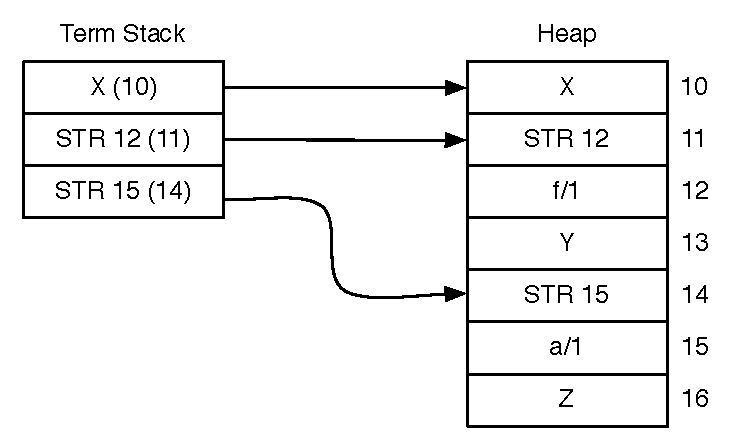
\includegraphics[scale=0.6]{lookup_subgoal_termstack_start.pdf}
  \caption{Initial term stack and heap representation for subgoal \texttt{p(X,f(Y),a(Z))}.}
  \label{fig:lookup_subgoal_termstack_start}
\end{figure}

The basic idea of this algorithm is to match the current term from the term stack against a node in the current
trie level and store the next alternative node on this level on the call choice point stack. If no node
is found, we try alternatives on the choice point stack, else we use the matched node to descend into the trie.
Two modes of matching exist: (1) \textbf{MATCH\_EXACTLY}, which is used when a new trie level is reached for the
first time in order to do exact matches; (2) \textbf{MATCH\_TRIE\_VARS}, used when the current trie node is reached
by backtracking, forcing variable matching.

\begin{figure}[ht]
\begin{Verbatim}
lookup_subsuming_call(subgoal_trie, subgoal_call) {
  match_mode = MATCH_EXACTLY
  path_type = VARIANT_PATH
  parent = trie_root(subgoal_trie)
  node = child(parent)
  var_chain = NULL
  push_arguments(term_stack, subgoal_call)

  while (!empty(term_stack))
    term = deref(pop(term_stack))
    push(term_log_stack, term)
  
    if (is_atom(term) or is_integer(term))
      match_node = match_constant_term(term, parent, node, var_chain, match_mode, path_type)
    else if (is_functor(term) or is_list(term))
      match_node = match_structured_term(term, parent, node, var_chain, match_mode, path_type)
    else if (is_variable(term))
      match_node = match_variable_term(term, parent, node, var_chain, match_mode, path_type)
  
    if (match_node == NULL)
      if (empty(call_choice_point_stack))   // no more alternatives
        return NO_PATH
      else
        match_mode = MATCH_TRIE_VARS   // backtrack mode
        (node, var_chain) = pop_call_choice_point_frame(call_choice_point_stack)
        parent = parent(node)
    else   // valid match, descend into node
      match_mode = MATCH_EXACTLY
      parent = match_node
      node = child(parent)
      
    return (path_type, parent)
}
\end{Verbatim}
\caption{Pseudo-code for procedure \texttt{lookup\_subsuming\_call}.}
\label{fig:lookup_subsuming_call}
\end{figure}

\subsection{Call Choice Point Stack}

The call choice point stack (Figure~\ref{fig:call_choice_point_stack}) contains alternative
search paths to use if the process fails somewhere in the trie.
Each stack frame can resume the search at a given node by restoring all the auxiliary stacks state at the time
of the call frame creation.

\begin{figure}[ht]
  \centering
    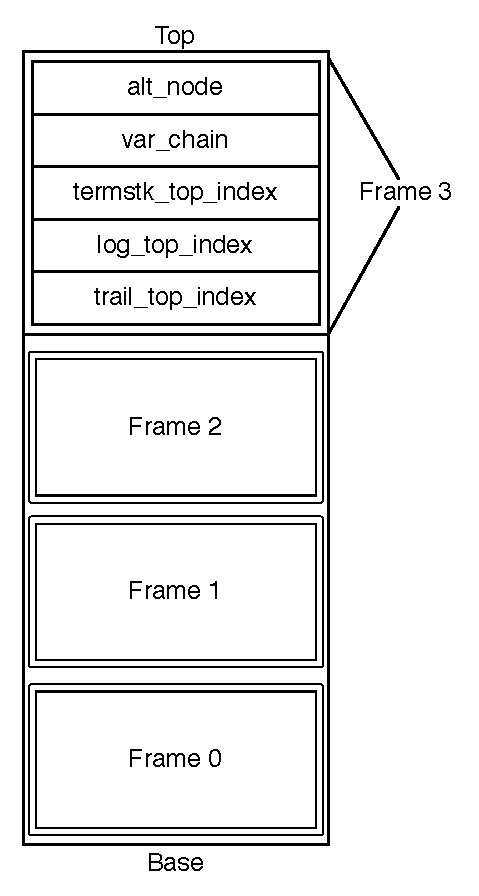
\includegraphics[scale=0.6]{call_choice_point_stack.pdf}
  \caption{Call choice point stack organization.}
  \label{fig:call_choice_point_stack}
\end{figure}

Each frame contains the next trie node to explore (\texttt{alt\_node}),
the current variable chain (\texttt{var\_chain}),
and the following stack indexes during frame creation:
the top of the term stack (\texttt{term\_stack\_top}),
the top of the term log stack (\texttt{term\_log\_stack\_top}),
and the top of the trail stack (\texttt{trail\_stack\_top}).

When popping a frame from the call choice point stack, the state of the auxiliary stacks and the other data
structures is restored. Consider a computational state $S_1$ pushed onto the stack
as frame $F1$. Given that we are at state $S_2$ and we need to backtrack to the previous state,
first we need to remove $F1$ from the stack and then we use the frame's information to restore $S_1$.

Any terms that were popped from the term stack from $S_1$ to $S_2$, which were
stored in the term log stack must be restored back into the term stack.
Then, any bindings made from $S_1$ to $S_2$ must be untrailed, which is
accomplished by \textit{unwinding} the trail stack. The unwind process untrails
the trie variables bound to the variable bindings vector
and the term variables which may have been made to point to the variable enumerator
vector. The node associated with state $S_2$ and its successors are never visited again and
the process continues until a leaf node is reached or the call choice point stack
is exhausted.

\subsection{Matching Constant Terms}

The \texttt{match\_constant\_term} procedure (Figure~\ref{fig:match_constant}) is called whenever the
next term from the term stack is an integer or an atom term.
First, the procedure checks if the match method is to exactly match the
sub-term constant against a trie symbol, which means
that this is the first time this trie level is explored (phase 1 in Figure~\ref{fig:match_constant}).
If the current trie level is represented by a simple linked list, both \texttt{node} and \texttt{var\_chain}
point to the start of the chain, but if the trie level is an hash table,
\texttt{node} will be made to point to the corresponding indexed bucket and \texttt{var\_chain}
to the variable bucket, which is always the first bucket. This is accomplished by the \texttt{set\_node\_and\_var\_chain}
procedure.

\begin{figure}[ht]
\begin{Verbatim}
match_constant_term(constant, parent, node, var_chain, match_mode, path_type) {
  // phase 1: try exact match
  if (match_mode == MATCH_EXACTLY)
    (node, var_chain) = set_node_and_var_chain(constant, node)
    match_node = find_matching_node(constant, node)
    if (match_node != NULL)
      conditionally_push_call_choice_point_frame(call_choice_point_stack, var_chain)
      return match_node
    else // no match found  
      no_variant_found(parent, path_type)
      node = var_chain
  // phase 2: no exact match, try bound trie variables
  match_node = find_bound_trie_var(constant, node)
  if (match_node != NULL)
    push_call_choice_frame(call_choice_point_stack, sibling(match_node), var_chain)
    return match_mode
  // phase 3: no bound trie variable, try unbound trie variables
  match_node = find_unbound_trie_var(var_chain)
  if (match_node != NULL)
    bind_trie_var(match_node, constant)
    return match_node
  return NULL
}
\end{Verbatim}
\caption{Pseudo-code for procedure \texttt{match\_constant\_term}.}
\label{fig:match_constant}
\end{figure}

The procedure \texttt{find\_matching\_node} iterates over a linked list and locates a trie node that matches the
\textbf{constant} symbol. When successful, we conditionally push a new call choice frame on the stack
with the first node from the variable chain that contains a trie variable
(\texttt{conditionally\_push\_call\_choice\_point\_frame}).
Note that only trie variables can be explored next as there is at most one node with the previously
matched symbol.

If an exact match fails, we know that no variant path exists for the called subgoal, and we use the
\texttt{no\_variant\_found} procedure to record the node from where the variant path can be
constructed and to mark the \texttt{path\_type} as \texttt{SUBSUMPTIVE\_PATH}.

Phase 2 of \texttt{match\_constant\_term} can be reached by a failed exact match or by backtracking
(remember that the match mode changes to \texttt{MATCH\_TRIE\_VARS} when backtracking). In this step
we call \texttt{find\_bound\_trie\_var} that will iterate over the \texttt{node} chain to look for
\textit{bound trie variables}. When traversing the subgoal trie, each new trie variable
along a path is marked, so it is easy to check for old variables, which have already been bound
to some term before arriving at the current node. The variable binding can be retrieved by
checking the variable bindings vector for the position corresponding to this variable
number, which points to an heap term. Given that we are trying to match a constant symbol,
we verify if the bound term matches our symbol. In this case, we create a new choice point
for the sibling node of the matched trie variable, and use the currently set variable chain.

Finally, if phases 1 and 2 fail, we try to match our constant against an unbound trie variable
(procedure \texttt{find\_unbound\_trie\_var}).
Phase 3 can be also reached by a failed exact and bound trie variable match or by subsequent backtrack
attempts. If a node is found, we trail the variable and its position on the variable bindings
vector is made to point to the constant term (procedure \texttt{bind\_trie\_var}).

\subsection{Matching Structured Terms}

When a structured term appears on the term stack, either a functor or a list, the matching
process works just like as for constants, except that the functor or list arguments are
pushed to the term stack after an exact match is found (Figure~\ref{fig:match_structured_term}).

\begin{figure}[ht]
\begin{Verbatim}
match_structured_term(term, parent, node, var_chain, match_mode, path_type) {
  // phase 1: try exact match
  if (match_mode == MATCH_EXACTLY)
    (node, var_chain) = set_node_and_var_chain(term, node)
    match_node = find_matching_node(term, node)
    if (match_node != NULL)
      push_arguments(term_stack, term)
      conditionally_push_call_choice_point_frame(call_choice_point_stack, var_chain)
      return match_node
    else // no match found
      no_variant_found(parent, path_type)
      node = var_chain
  // phase 2: no exact match, try bound trie variables
  match_node = find_bound_trie_var(term, node)
  if (match_node != NULL)
    push_call_choice_frame(call_choice_point_stack, sibling(match_node), var_chain)
    return match_node
  // phase 3: no bound trie variable, try unbound trie variables
  match_node = find_unbound_trie_var(var_chain)
  if (match_node != NULL)
    bind_trie_var(match_node, term)
    return match_node
  return NULL
}
\end{Verbatim}
\caption{Pseudo-code for procedure \texttt{match\_structured\_term}.}
\label{fig:match_structured_term}
\end{figure}

Figure~\ref{fig:match_functor} shows the evolution of the term stack for finding
a subsuming goal for subgoal \texttt{p(a,f(b))}. Step 1 shows the initial
term stack, followed by the match of the term on top of the stack, \texttt{a},
against the trie node $n1$, \texttt{VAR0}.
Being an unbound trie variable, the first position of the variable bindings
vector is thus bound to \texttt{a}.
Next, we try to match the functor \texttt{f/1} against node $n2$, but we fail (step 2).
Then, node $n3$ succeeds, as it is an exact match, and the functor argument \texttt{b} is pushed on
the term stack (step 3). Finally, \texttt{b} matches against node $n4$, and we find
a subsuming call: \texttt{p(VAR0,f(b))}.

\begin{figure}[ht]
  \centering
    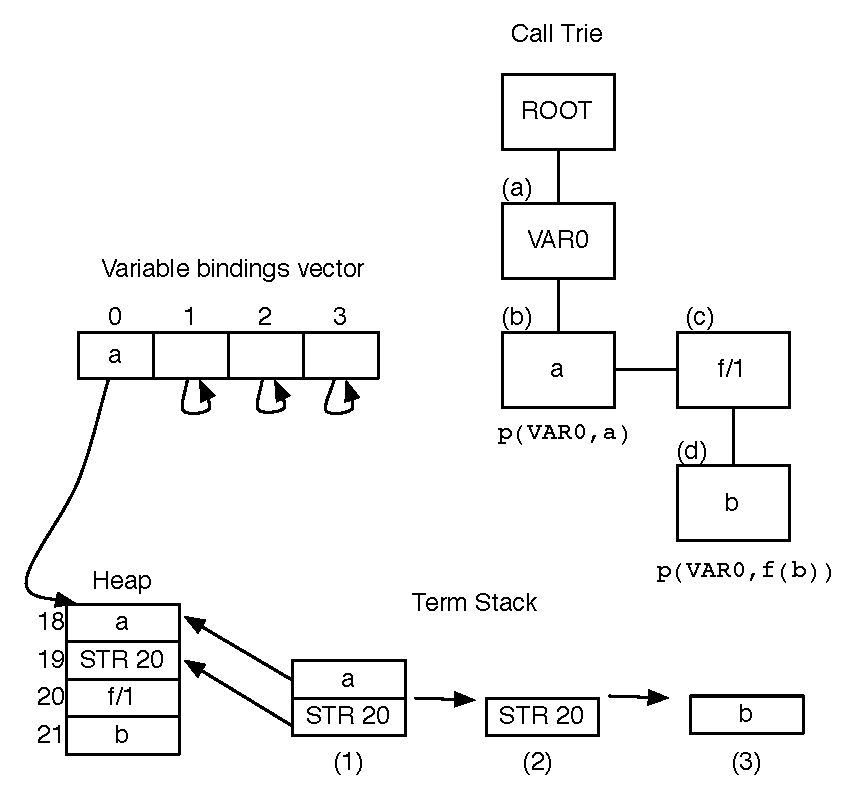
\includegraphics[scale=0.6]{match_functor.pdf}
  \caption{Finding a subsuming goal for subgoal \texttt{p(a,f(b))}.}
  \label{fig:match_functor}
\end{figure}

\subsection{Matching Variable Terms}

The last case for the matching algorithm are variable terms. Because we are trying to find a more general goal,
a term variable must only be matched or bound against a trie variable and a
never seen variable must match only with an unbound trie variable.

Consider the case of trying to match \texttt{p(X,Y)} against \texttt{p(VAR0,VAR0)}.
The first call variable \texttt{X} could match the first trie variable \texttt{VAR0},
but then the call variable \texttt{Y} must be matched against an unbound variable and
thus the trie variable \texttt{VAR0} cannot be used, because it
was already bound to variable \texttt{X}.

To recognize already seen call variables, we bind them to the variable enumerator vector, indexed
by the corresponding trie variable number. The trail stack is used to trail those variables.
When a bound variable must be matched again, first we try to pair it with the same trie variable,
and if such trie variable can not be found, we try an unbound trie variable, thus,
avoiding two different call variables to be bound to the same trie variable.

The pseudo-code for this procedure is shown in Figure~\ref{fig:match_variable}.
From it, we can conclude that a variant path
cannot be found when:
(1) we cannot match an already seen call variable against the same trie variable already bound to it;
or (2) a new trie variable cannot be found for a new call variable.

\begin{figure}[ht]
\begin{Verbatim}
match_variable_term(variable, parent, node, var_chain, match_mode, path_type) {
  if (match_mode == MATCH_EXACTLY)
    (node, var_chain) = set_node_and_var_chain(variable, node)
    if (!is_in_variable_enumerator_vector(variable))
      // variable not seen before
      foreach (match_node in node)
        if (is_trie_var(match_node) and is_new_variable(match_node))
          // only one new trie variable per level, no choice point needed
          bind_trie_var(match_node, variable)
          mark_variable_enumerator_vector(variable, var_index(match_node))
          return match_node
      no_variant_found(parent, path_type)
      return NULL
  // variable has been seen before
  foreach (match_node in node)
    if (is_trie_var(match_node) and !is_new_variable(match_node))
      if (identical_terms(trie_var_bindings[match_node], variable))
        push_call_choice_frame(call_choice_point_stack, sibling(match_node), var_chain)
        return match_node
  // variant path is not possible here
  no_variant_found(parent, path_type)
  // match against unbound trie variable
  foreach (match_node in var_chain)
    if (is_trie_var(match_node) and is_new_variable(match_node))
      // only one new trie variable per level, no choice point needed
      bind_trie_var(match_node, trie_var_bindings[prolog_var_index(variable)])
      return match_node
  return NULL
}
\end{Verbatim}
\caption{Pseudo-code for procedure \texttt{match\_variable\_term}.}
\label{fig:match_variable}
\end{figure}

\subsection{Variant Continuations}

A \textit{variant continuation} is built when the algorithm detects that a variant path of the
called subgoal cannot be found on the subgoal trie during the search process.
A variant continuation stores all the needed information to later resume
the algorithm that creates the variant path. This includes the node from where the rest of the variant
path is created (i.e., the last node from where the search for a variant path was still valid),
the term stack and all the bindings made to the call variables that were trailed on the trail stack.
In previous pseudo-code listings we used the procedure \texttt{no\_variant\_found} to do that.
This procedure creates a variant continuation the first time it is called.

Figure~\ref{fig:variant_continuation} shows a variant continuation that is built
after the match process failed at node \texttt{c}. If a variant path
for subgoal \texttt{p(X,f(Y),b)} needs to be created, the following must be done:
(1) the term stack is restored with the terms saved on the continuation;
(2) the trail stack is initialized with
the two variable heap addresses and each variable is bound to the saved
enumerator addresses. The variable enumerator vector is used during the insertion
of variant paths to detect if a variable was already seen and easily compute its number by
looking at the enumerator position.

\begin{figure}[ht]
  \centering
    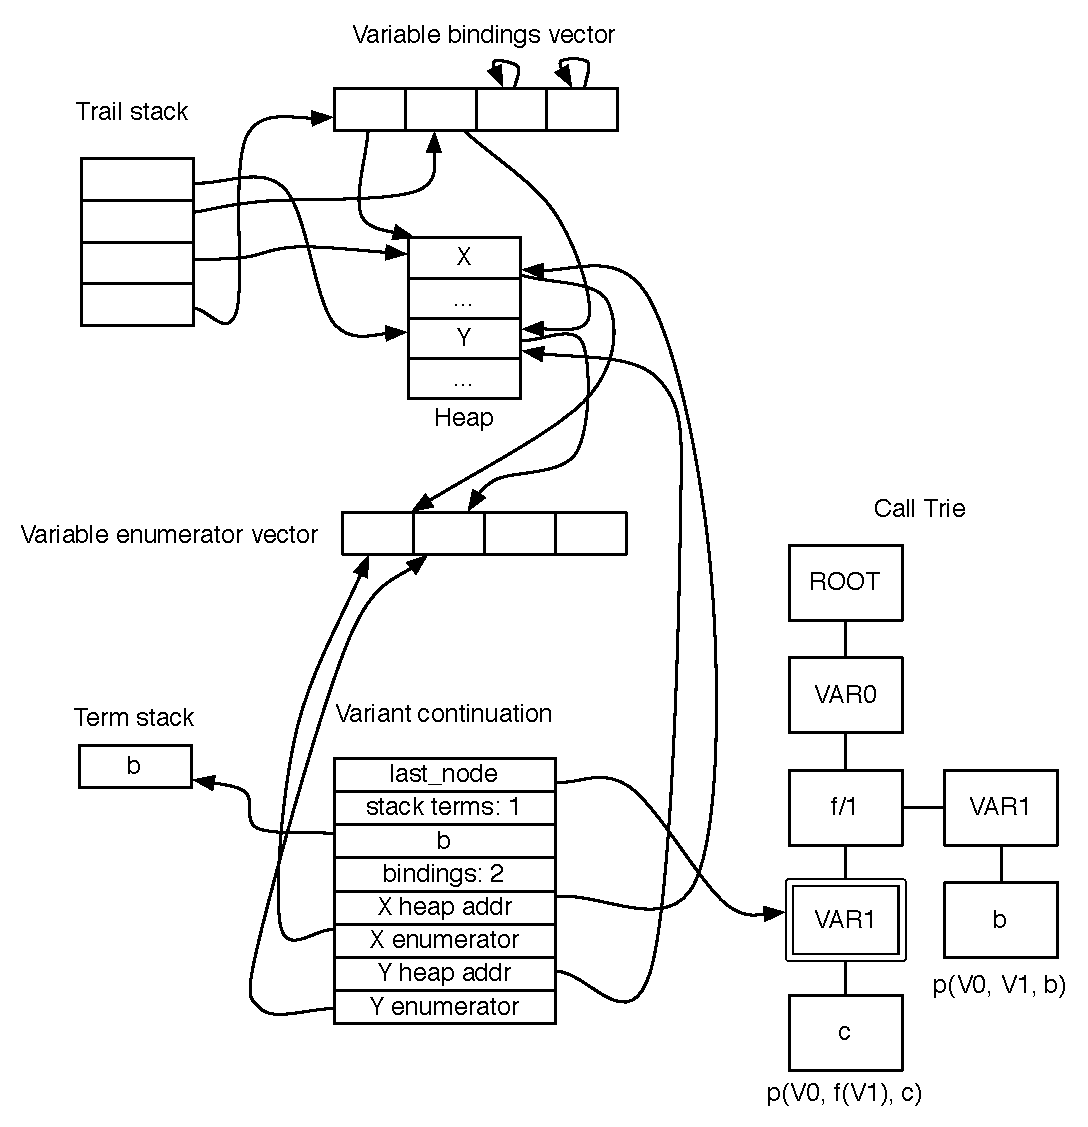
\includegraphics[scale=0.6]{variant_continuation.pdf}
  \caption{Variant continuation for subgoal \texttt{p(X,f(Y),b)}.}
  \label{fig:variant_continuation}
\end{figure}

\section{Answer Templates}

In a variant engine, the substitution factor \cite{RamakrishnanIV-95}
represents the variables which exist in the terms of the argument registers.
These variables are dereferenced when inserting answers in an answer trie (for general calls)
or bound to terms when consuming answers from an answer trie (for consumer calls).
Figure~\ref{fig:answer_template_generator} shows how a substitution factor is constructed
on the local stack associated with a generator choice point.
Note that the substitution factor size (2) in the example is also stored.

\begin{figure}[ht]
  \centering
    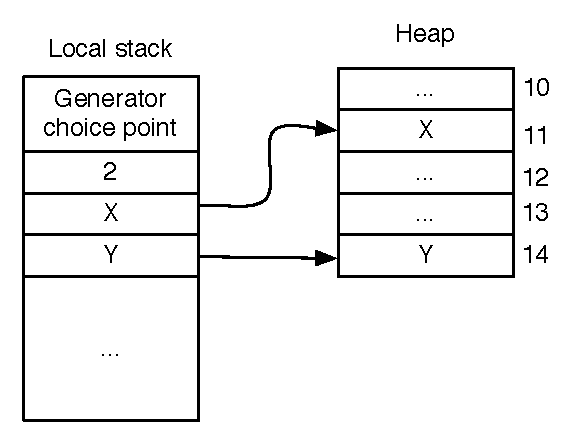
\includegraphics[scale=0.6]{answer_template_generator.pdf}
  \caption{Substitution factor for \texttt{p(X,f(Y))}.}
  \label{fig:answer_template_generator}
\end{figure}

When using call by subsumption, the same factor is used for subgoals which do not
consume from more general subgoals, i.e., generator subgoals or variants of generator
subgoals. We call this type of substitution factor a \textit{generator answer template}.

For subgoals with more general subgoals, subsumed subgoals or variants of subsumed subgoals,
the answer template must specialize the generator answer template
from the most general subgoal, and is called a \textit{consumer answer template}.
Consumer answer templates have the exact same size of their corresponding generator answer templates
and instead of being composed only with variables, they can also include other types of sub-terms.

Consider a generator subgoal \texttt{p(X,f(Y))} and that the subgoal \texttt{p(a,f(g(2,X)))}
is then called. The corresponding answer template \texttt{[a,~g(2,X)]} is derived by instantiating
the generator variables, \texttt{X} and \texttt{Y}, with the terms in the consumer subgoal
(see Figure~\ref{fig:answer_template_consumer}).

\begin{figure}[ht]
  \centering
    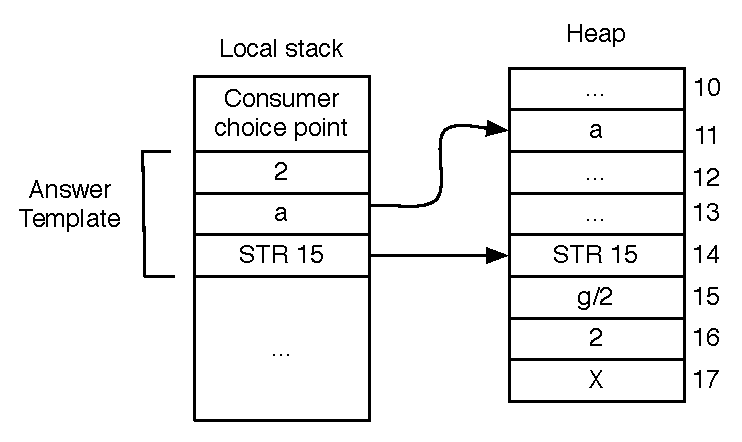
\includegraphics[scale=0.6]{answer_template_consumer.pdf}
  \caption{Consumer answer template for \texttt{p(a,f(g(a,X)))}.}
  \label{fig:answer_template_consumer}
\end{figure}

The construction of answer templates is done when searching the subgoal trie for a more general goal.
If no subsuming subgoal is found, then a generator answer template is built. If a subsuming subgoal
exists, then the found subgoal frame $S$ can be either:

\begin{enumerate}
  \item a generator subgoal frame: the answer template is built using
  the variable bindings vector as shown in procedure \textbf{construct\_answer\_template\_from\_lookup}
  (Figure~\ref{fig:construct_answer_template_from_lookup});
  
  \item a consumer subgoal frame: the answer template is reconstructed by using the generator
  subgoal frame of $S$ as we consume only from proper generators. 
  The procedure \texttt{construct\_answer\_template\_from\_generator}
  (Figure~\ref{fig:construct_answer_template_from_generator}) builds this answer template by
  matching new trie variables against terms from the specific subgoal. It
  uses another stack, the \textit{symbol stack}, to push the trie
  symbols from the general subgoal path. The term stack is used to push the called subgoal arguments that
  will be matched against the trie symbols. Note that when a functor or list symbol appears
  on the symbol stack the current term is also certainly a functor or list, because the called subgoal
  specializes the more general subgoal.
\end{enumerate}

\begin{figure}[ht]
\begin{Verbatim}
construct_answer_template_from_lookup() {
  total = 0
  foreach (binding in variable_bindings_vector)
    total++
    answer_template[total] = binding
  answer_template[0] = total
  return answer_template
}
\end{Verbatim}
\caption{Pseudo-code for procedure \texttt{construct\_answer\_template\_from\_lookup}.}
\label{fig:construct_answer_template_from_lookup}
\end{figure}

\begin{figure}[ht]
\begin{Verbatim}
construct_answer_template_from_generator(subgoal_call, generator_sf) {
  push_trie_path(symbol_stack, subgoal_trie_path(generator_sf))
  push_arguments(term_stack, subgoal_call)
  
  total = 0
  while (!empty(term_stack))
    term = deref(pop(term_stack))
    symbol = pop(symbol_stack)
    if (is_trie_var(symbol) and is_new_variable(symbol))
      total++
      answer_template[total] = term
    else if (is_functor(symbol) or is_list(symbol))
      push_arguments(term_stack, term)
  
  answer_template[0] = total
  return answer_template
}
\end{Verbatim}
\caption{Pseudo-code for procedure \texttt{construct\_answer\_template\_from\_generator}.}
\label{fig:construct_answer_template_from_generator}
\end{figure}

\section{Time Stamped Answer Trie}

A time stamped node extends an answer trie node with time stamp information.
Each node contains the following fields: \textbf{symbol}, \textbf{child}, \textbf{parent}, \textbf{sibling}
and \textbf{timestamp}. For implementation and algorithmic purposes, each node also needs a bit field,
\textbf{status}, that defines some node properties that will be described shortly.

Insertion of an answer $S$ into a TST can be divided into two steps:

\begin{enumerate}
  \item Finding a more general answer $S'$ on the trie.
  \item Inserting $S$ if $S'$ could not be found.
\end{enumerate}

To implement step 1, we use the same algorithm described in Section \ref{sec:lookup_subsuming}
but now to search for a \textit{more general answer} or a \textit{repeated answer} (i.e., a variant of $S$).
If step 1 fails, step 2 then uses the variant continuation to resume the insertion of the answer
on the last node where the variant answer path was still expected to be found during step 1.

\begin{figure}[ht]
\begin{Verbatim}
subsumptive_answer_search(trie_root, ans_vector)
  (path, leaf) = lookup_subsuming_call(trie_root, ans_vector) // step 1
  if (path == NO_PATH)
    // step 2
    node = restore_variant_continuation()
    leaf = tst_insert(trie_root, node)
  return leaf
}
\end{Verbatim}
\caption{Pseudo-code for procedure \texttt{subsumptive\_answer\_search}.}
\label{fig:subsumptive_answer_search}
\end{figure}

The procedure \texttt{subsumptive\_answer\_search} (Figure~\ref{fig:subsumptive_answer_search})
implements this process and needs two arguments: the root of the answer trie \texttt{trie\_root}, and
the answer as a vector of terms, \texttt{ans\_vector}.

When a chain of sibling nodes becomes larger than a threshold value, we dynamically index the
nodes through an hash table to provide direct node access and therefore optimize the search. Given
that an hash table can have a large number of answer nodes with different time stamp values, we maintain
a reference to these nodes, in decreasing order of their time stamp values in a double linked list
called the \textit{time stamped index}.
Besides the double linked list pointers, each index node contains a pointer to the corresponding
answer node and the value of its time stamp. Each answer node indexed in the hash table has a different use
for the \textbf{timestamp} field: instead of containing a positive integer, contains a pointer
to the respective index node. The trie node field \textbf{status} distinguishes
both cases. Figure~\ref{fig:hash_table_tst} illustrates an hash table with a time stamp index.

\begin{figure}[ht]
  \centering
    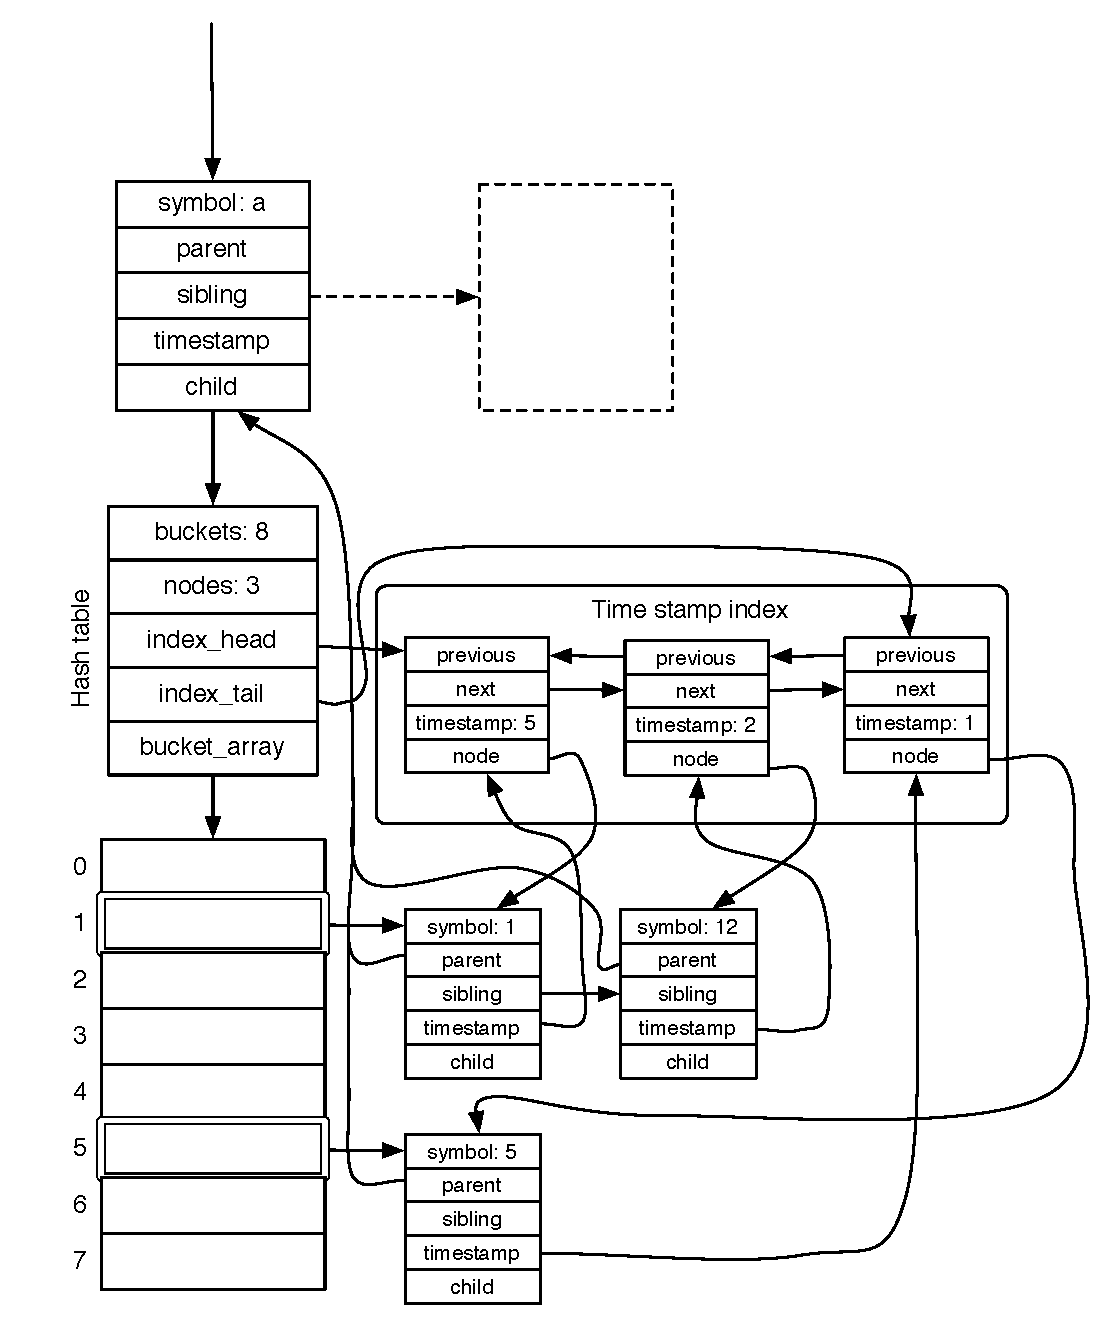
\includegraphics[scale=0.6]{hash_table_tst.pdf}
  \caption{Indexing nodes through an hash table with time stamp indexes.}
  \label{fig:hash_table_tst}
\end{figure}

\subsection{Inserting New Answers}

Once the variant continuation is restored, the rest of the answer path can be inserted on the trie starting
from the restored node. Inserting is then a simple operation because no checking for equal trie symbols is required.
The first symbol will be inserted either into: (1) a childless parent node (i.e., the trie root);
(2) a parent node pointing to a sibling chain list; (3) a parent node pointing to an hashed child node.
Every other symbols will be inserted on childless parents.

Procedure \texttt{tst\_insert} (Figure~\ref{fig:tst_insert}) does the job of inserting
all the terms contained in a stack of terms into the trie, starting from \texttt{node}.
The difference between procedures \texttt{tst\_add\_symbol} and \texttt{tst\_insert\_symbol}
is that the former inserts symbols on childless nodes and the later on nodes with children.

\begin{figure}[ht]
\begin{Verbatim}
tst_insert(trie_root, node) {
  symbol = process_term_stack(term_stack)
  if (child(node) == NULL)
    // inserting on the root
    node = tst_add_symbol(node, symbol)
  else if (is_hash_table(node))
    node = tst_hash_table_add_symbol(node, symbol)
  else
    node = tst_insert_symbol(node, symbol)
  
  // at this point, just add nodes on childless parents
  while (!empty(term_stack))
    symbol = process_term_stack(term_stack)
    node = tst_add_symbol(node, symbol)
  
  update_timestamps(trie_root, node)
  return node
}
\end{Verbatim}
\caption{Pseudo-code for procedure \texttt{tst\_insert}.}
\label{fig:tst_insert}
\end{figure}

The procedure \texttt{process\_term\_stack} pops a term from the term stack and converts the term
to a trie representation, which is usually called a \textit{symbol}. If the term is a functor or a list,
the arguments are pushed into the stack of terms to be processed next.

While appending a new node in a sibling list does not involve any
time stamp indexing (see Figure~\ref{fig:tst_chain_insert}), inserting a new node into an hash table does,
because hash tables index nodes by time stamp.
Figure~\ref{fig:hash_table_insert}
illustrates the insertion of a symbol (\texttt{25}) and the creation of the respective
index node. Note that the \textbf{index\_head} field was changed to point to the new index node,
which is always the node with the greatest time stamp.

\begin{figure}[ht]
  \centering
    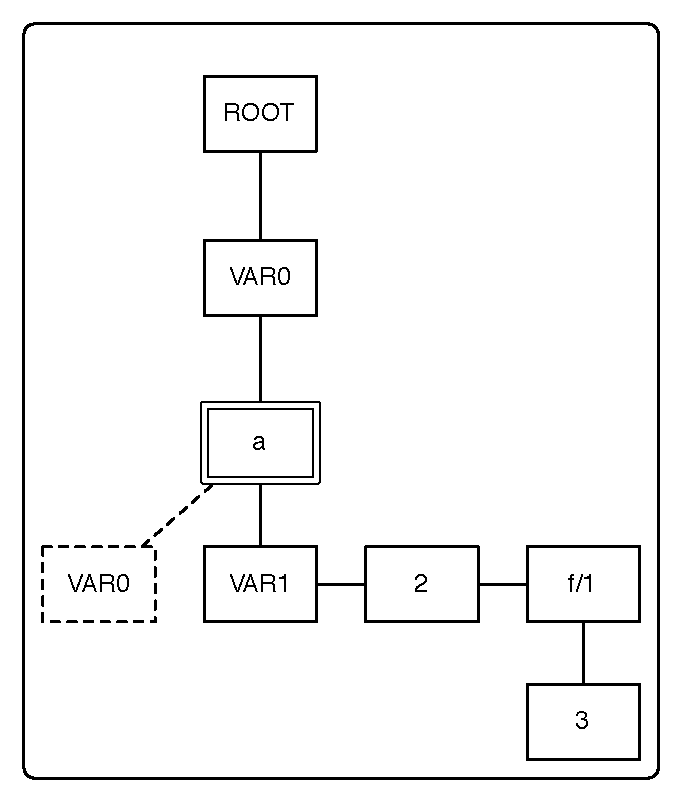
\includegraphics[scale=0.45]{tst_insert.pdf}
  \caption{Inserting answer $\{$\texttt{VAR0,a,VAR0}$\}$.}
  \label{fig:tst_chain_insert}
\end{figure}

\begin{figure}[ht]
  \centering
    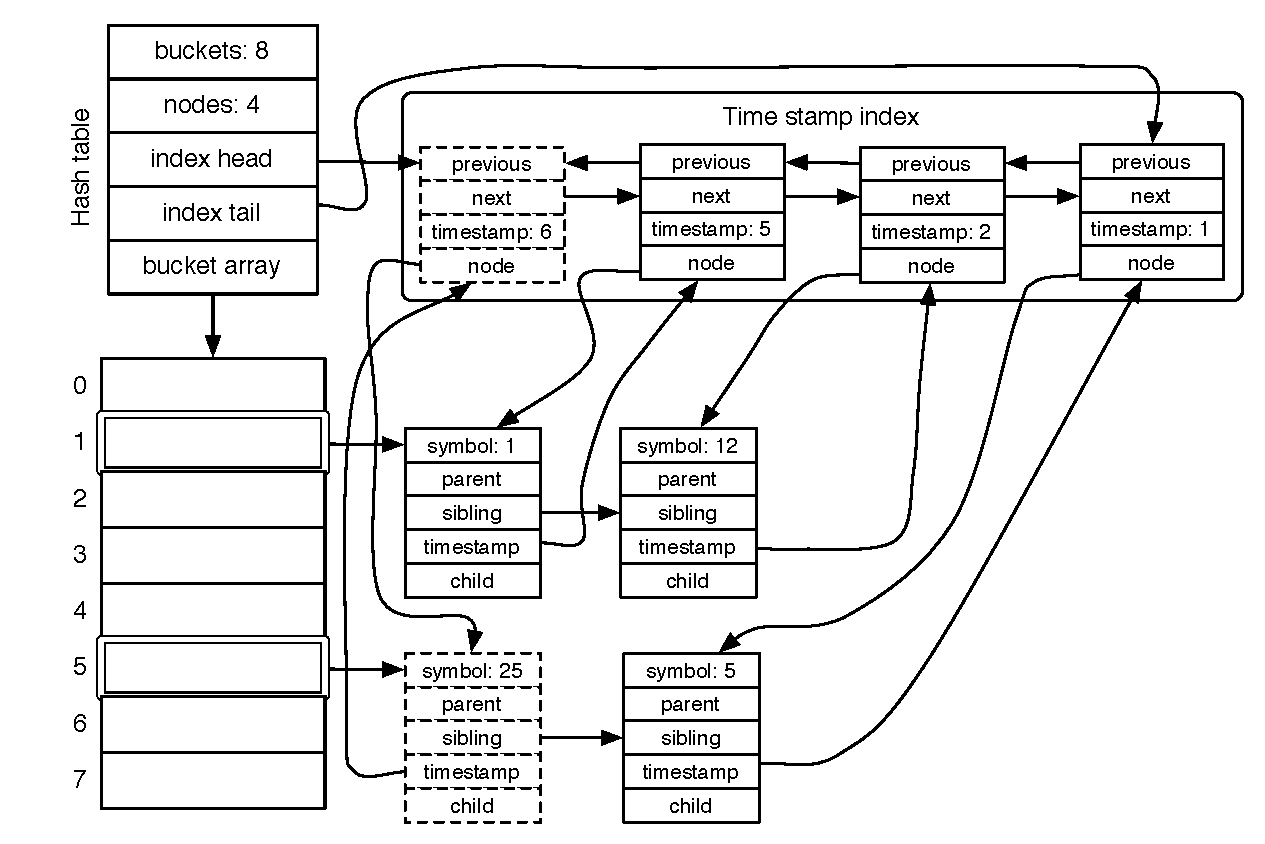
\includegraphics[scale=0.6]{hash_table_insert.pdf}
  \caption{Inserting a node into the hash table and updating the index.}
  \label{fig:hash_table_insert}
\end{figure}

\subsection{Updating Time Stamps}

Once an answer is inserted, the time stamps must be updated.
The time stamp for the new answer is calculated by inspecting the time stamp of the trie root node.
Next, we update the time stamps in the answer trie branch starting from the answer leaf node to the
root node.

If the current node is an hashed node with time stamp indexes,
its index node is moved to the head of
the index's double linked list. We can test whether an answer node is indexed by
an hash table by inspecting its \textbf{status} field.
Figure~\ref{fig:update_timestamps} contains the pseudo-code for procedure \texttt{update\_timestamps}.

\begin{figure}[ht]
\begin{Verbatim}
update_timestamps(trie_root, leaf) {
  new_timestamp = timestamp(trie_root) + 1
  
  while (leaf != trie_root)
    if (is_hashed_node_with_time_stamp_indexes(leaf))
      // relocate index node
      promote_entry(leaf, new_timestamp)
    else
      timestamp(leaf) = new_timestamp
    leaf = parent(leaf)
      
  timestamp(trie_root) = new_timestamp
}
\end{Verbatim}
\caption{Pseudo-code for procedure \texttt{update\_timestamps}.}
\label{fig:update_timestamps}
\end{figure}

When moving an index node $N$, the \textbf{index\_head} field of the hash table must be updated
to point to $N$. Moreover, if $N$ was at the end of the chain,
the \textbf{index\_tail} field must be also updated to the \textbf{previous} field of $N$.
Previous pointers of the \textbf{next} node of $N$ and the next pointer of
the \textbf{previous} node of $N$ must
also be updated to keep the chain consistent.
Figure~\ref{fig:hash_table_promote} illustrates the relocation of an index node, after
its time stamp be updated from 5 to 7.

\begin{figure}[ht]
  \centering
    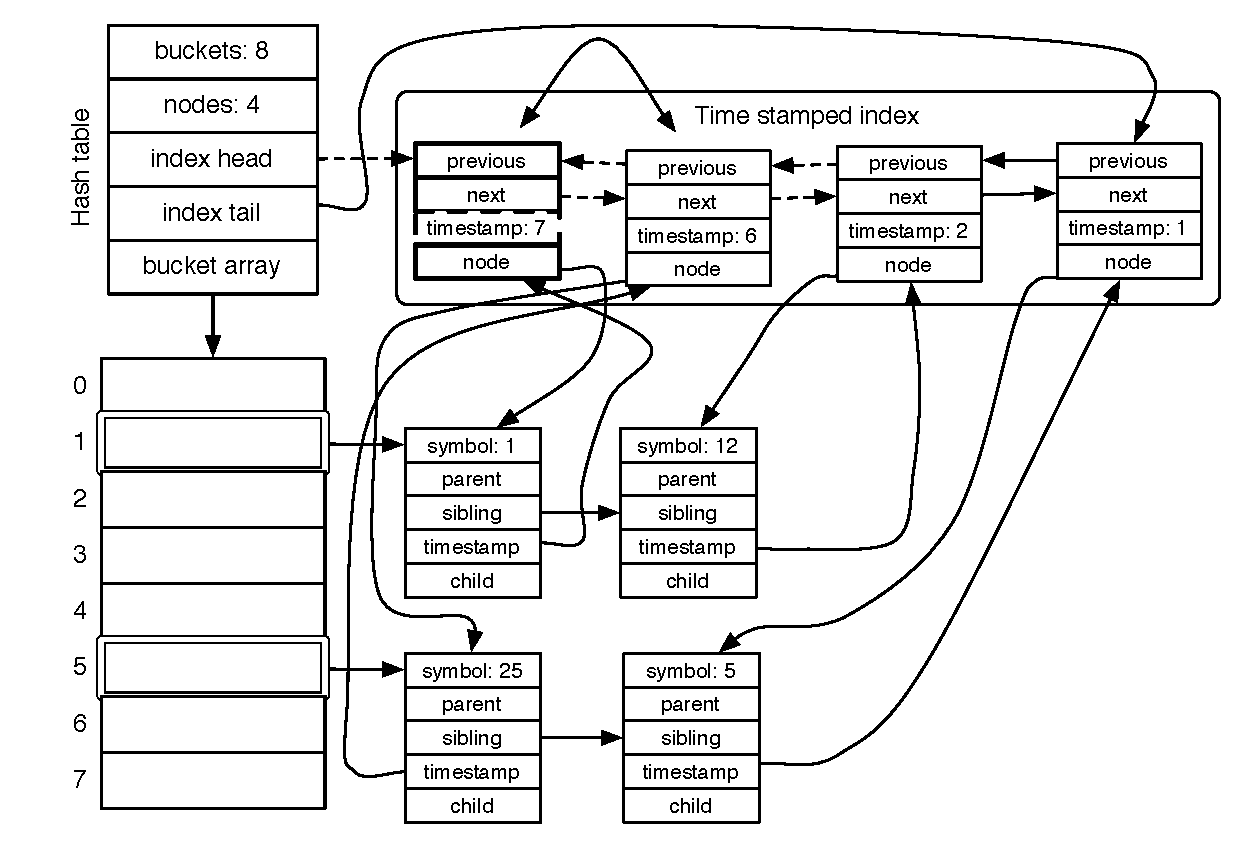
\includegraphics[scale=0.6]{hash_table_promote.pdf}
  \caption{Promoting an index node.}
  \label{fig:hash_table_promote}
\end{figure}

\subsection{Lazy Creation of Time Stamp Indexes}

Time stamped indexes are only created when a consumer subgoal is first called.
We must iterate over all the hash tables present on the trie to create the time stamp index.
To efficiently locate all hash tables in an answer trie, we chain these hash tables
using the \textbf{next} field and the start of this chain is stored
in the \textbf{sibling} field of the root node.

Creating the index for an hash table amounts to iterating over the hashed nodes
and orderly inserting new index nodes on the index chain.
Later, when the subgoal completes, the time stamp indexes can be thrown away to save space,
because they are only necessary during collection of relevant answers for consumer subgoals.

\section{Collecting Relevant Answers}\label{sec:collect}

The process of collecting relevant answers for a consumer subgoal $G$ from an answer trie $T$
of the generator subgoal $G'$, involves searching $T$ for a set $S$ of answers that unify
with the consumer answer template $AT$ and are newer than the time stamp
$TS$ stored in the consumer subgoal frame. After collection, $TS$ is updated to the
time stamp of the root node of $T$, thus avoiding repeated answers in future iterations
of the algorithm. Collected answers are then appended to the list of answers of the consumer
subgoal frame, so that they can be reused in future calls of $G$.

Various data structures are used for this algorithm, namely:

\begin{itemize}
  \item \textit{WAM data structures}: the push down list (PDL),
  heap, trail, and associated registers. The heap is used to build structured terms, in which the
  answer template or trie variables are bound. Whenever a variable is bound, we trail it using the WAM trail. The \textit{unify} operation provided by the WAM is used to check for term equality in structured terms;
  
  \item \textit{term stack}: used to store the next terms to be processed as we navigate through the time
   stamped trie $T$;
  
  \item \textit{term log stack}: when an unification fails, there is a need to backtrack to inspect other
  alternative branches. This stack is used to store already processed terms of the term stack,
  so they can be restored back during backtracking;
  
  \item \textit{variable bindings vector}: stores the bindings for the trie variables;
  
  \item \textit{choice point stack}: stores choice point frames, where each frame contains
  information needed to restore the computation in order to search for alternative branches.
\end{itemize}

The pseudo-code for the algorithm is presented in Figure~\ref{fig:tst_collect_relevant_answers}.
The whole algorithm can be summarized into eight steps:

\begin{enumerate}
  \item Setup phase: setup term stack and WAM machinery.
  \item Fetch a term $T$ from the term stack;
  \item Search for a node $N$ at the current trie level that has a valid time stamp;
  \item Search for the next valid node to be pushed on the choice point stack;
  \item Unify $T$ with the trie symbol of $N$;
  \item Proceed into the child of $N$ or, if steps 3 or 5 fail, backtrack by popping a frame from the choice point stack and use the alternative node to unify;
  \item Once a leaf is reached, mark it as a new answer and possibly backtrack to retrieve more answers.
  \item If no more choice point frames exist, return the marked answers.
\end{enumerate}

The setup phase pushes the answer template into the term stack and backups the WAM registers.
The trail register is set to the next free position
of the WAM trail, thus avoiding writing on frozen segments. Registers HB, H and TR are
saved as they will be manipulated and need to be restored to avoid any interference with
the normal WAM execution.

\begin{figure}[ht]
\begin{Verbatim}
tst_collect_relevant_answers(trie_root, ts, answer_template) {
  answers = NULL
  push_terms(term_stack, answer_template)
  save_wam_registers()
  parent = trie_root
  node = child(parent)
  
while_loop:
  while (!empty(term_stack))
    term = deref(pop(term_stack))
    
    if (is_atom(term) or is_integer(term))
      unify_node = unify_constant_term(term, node, ts)
    else if (is_functor(term) or is_list(term))
      unify_node = unify_structured_term(term, node, ts)
    else if (is_variable(term))
      unify_node = unify_variable_term(term, node, ts)
      
    if (unify_node != NULL)
      parent = unify_node
      node = child(parent)
      continue
    else if (empty(choice_point_stack))
      unwind_wam_trail()
      restore_wam_registers()
      return answers
    else
      node = pop_choice_point_frame(choice_point_stack)
      parent = parent(node)
  
  new_answer_found(parent, answers)
  if (empty(choice_point_stack)
    unwind_wam_trail()
    restore_wam_registers()
    return answers
  node = pop_choice_point_frame(choice_point_stack)
  parent = parent(node)
  goto while_loop
}
\end{Verbatim}
\caption{Pseudo-code for procedure \texttt{tst\_collect\_relevant\_answers}.}
\label{fig:tst_collect_relevant_answers}
\end{figure}

\subsection{Choice Point Stack}\label{sec:cpstack_section}

The choice point stack stores alternative search branches to use upon backtracking.
Each stack frame (see Figure~\ref{fig:choice_point_stack}) stores the following fields:
\texttt{alt\_node}, the alternative node to explore;
\texttt{term\_stack\_top}, the top of the term stack;
\texttt{term\_log\_stack\_top}, the top of the term log stack;
\texttt{trail\_top}, the current trail position;
and \texttt{saved\_HB}, the register HB.

\begin{figure}[H]
  \centering
    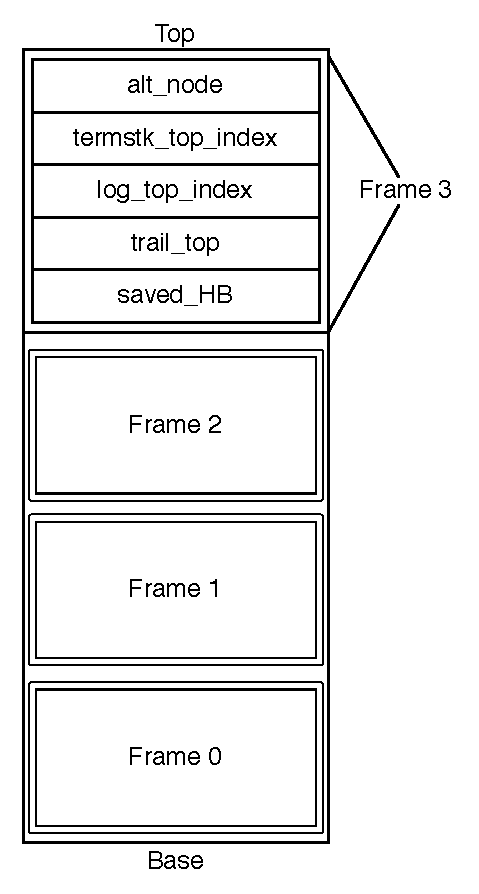
\includegraphics[scale=0.45]{choice_point_stack.pdf}
  \caption{Choice point stack organization.}
  \label{fig:choice_point_stack}
\end{figure}

The HB register serves the same purpose as the standard HB register in a WAM choice point.
During execution, the WAM's HB register is compared against the value of H to determine
if a variable is \textit{conditional}, that is, if a variable needs to be trailed, so that
when execution backtracks to a previous choice
point we can reset variable bindings. In our case, instead of executing WAM code, we unify a time stamped node,
thus the meaning of a conditional variable is extended to include the trie variables in the variable bindings vector.

When a choice point frame is popped from the stack, the state of the computation is resumed
by executing the following actions:

\begin{itemize}
  \item the current node and parent node are reset;
  \item all terms stored in the term log stack are pushed back to the term stack;
  \item the trail is unwound to reset the variables that were bound after choice point creation;
  \item registers H and HB are also reseted to previous values.
\end{itemize}

\subsection{Unification of Constant Terms}

Once a trie node $N$ is reached we must select the next trie node $N'$ that unifies with our
term and has a valid time stamp. Node $N$ can lead either to a simple node chain or an hash table.
With constant terms we can index the hash table to prune the search space
(procedure \texttt{set\_match\_and\_unify\_chains} in Figure~\ref{fig:unify_constant_term})
by using the \textit{match bucket}.

\begin{figure}[ht]
\begin{Verbatim}
unify_constant_term(constant, node, ts) {
  if (is_hash_table(node))
    // retrieve the indexed and variable buckets
    (match_chain, unify_chain) = set_match_and_unify_chains(constant, node)
    if (match_chain != unify_chain)
      node = search_chain_exact_match(constant, match_chain, unify_chain, ts)
      if (node != NULL)
         return node
      // exact match failed
      node = unify_chain
    if (node == NULL)
      return NULL
  return search_chain_unify_with_constant(constant, node, ts)
}
\end{Verbatim}
\caption{Pseudo-code for procedure \texttt{unify\_constant\_term}.}
\label{fig:unify_constant_term}
\end{figure}

Because variables can unify with the constant term, there is a need to retrieve the variable chain
(from the variable bucket), which will be used as the alternative chain to push on the choice point stack.
We call this chain the \textit{unify chain}. If the constant is found on the match chain,
the unify chain is used as alternative, but if no match was found, the variable chain will be attempted
next and, depending on the remaining nodes, also be used as the backtracking alternative.

\begin{figure}[ht]
\begin{Verbatim}
search_chain_exact_match(term, match_chain, unify_chain, ts) {
  foreach (node in match_chain)
    if (term == symbol(node))
      if (valid_timestamp(timestamp(node), ts))
        push_choice_point_frame(choice_point_stack, next_valid_node(unify_chain, ts))
        push(term_log_stack, term)
        return node
      else
        return NULL
  return NULL
}
\end{Verbatim}
\caption{Pseudo-code for procedure \texttt{search\_chain\_exact\_match}.}
\label{fig:search_chain_exact_match}
\end{figure}

In Figure~\ref{fig:unify_constant_term} we present the pseudo-code for procedure
\texttt{unify\_constant\_term}. First, we check for an hash table and inspect the match
bucket using \texttt{search\_chain\_exact\_match} (Figure~\ref{fig:search_chain_exact_match}).
Next, if no match is found we execute \texttt{search\_chain\_unify\_with\_constant}
(Figure~\ref{fig:search_chain_unify_with_constant}) on the unify chain. Otherwise, if no hash table
is found, we would consider the simple chain of sibling nodes as the unify chain and simply
execute \texttt{search\_chain\_unify\_with\_constant} on it.

\begin{figure}[ht]
\begin{Verbatim}
search_chain_unify_with_constant(constant, chain, ts) {
  chain = next_valid_node(chain, ts)
  while (chain != NULL)
    alt_chain = chain_next_valid_node(sibling(chain), ts)
    symbol = trie_deref(symbol(chain))
    if (is_variable(symbol)) // case (1)
      push_choice_point_frame(choice_point_stack, alt_chain)
      bind_and_conditionally_trail(symbol, constant)
      push(term_log_stack, constant)
      return chain
    else if (symbol == constant) // case (2)
      // exact match
      push_choice_point_frame(choice_point_stack, alt_chain)
      push(term_log_stack, constant)
      return chain
    else
      chain = alt_chain
  }
  // case (3)
  return NULL
}
\end{Verbatim}
\caption{Pseudo-code for procedure \texttt{search\_chain\_unify\_with\_constant}.}
\label{fig:search_chain_unify_with_constant}
\end{figure}

When searching the unify chain, first we locate the next node with a valid time stamp on the chain, that is,
with the time stamp greater than our target time stamp. Next, we \textit{dereference} the node symbol by using
\texttt{trie\_deref}, which returns a position on the variable bindings vector if the node symbol
is a trie variable, hence allowing trie variables to be used as \textit{normal} variables.

In case (1), a variable was found, which can be a position on the variable bindings vector or a Prolog
variable that was bound to a trie variable. Either way, we bind the variable to the constant term,
push a new choice point frame with the next valid node, and return \texttt{chain} to be explored next.
Please note that the procedure \texttt{bind\_and\_conditionally\_trail} tests if the variable (first argument)
is a conditional variable and then trails it using the WAM trail.

In case (2) the node symbol matches our constant and we simply push a new choice point frame and advance
into the next node.

Otherwise, if we could not found a valid trie node in the unify chain, we get into case (3), and the choice point
stack must be used to try alternatives.

As an example, let's consider the time stamped trie in Figure~\ref{fig:tst_constant_a}. The input
answer template is $\{$\texttt{a,b,b}$\}$ and the target time stamp is 3.

\begin{figure}
   \centering
   
   \subfloat[Time stamped trie.]{%
      \label{fig:tst_constant_a}%
      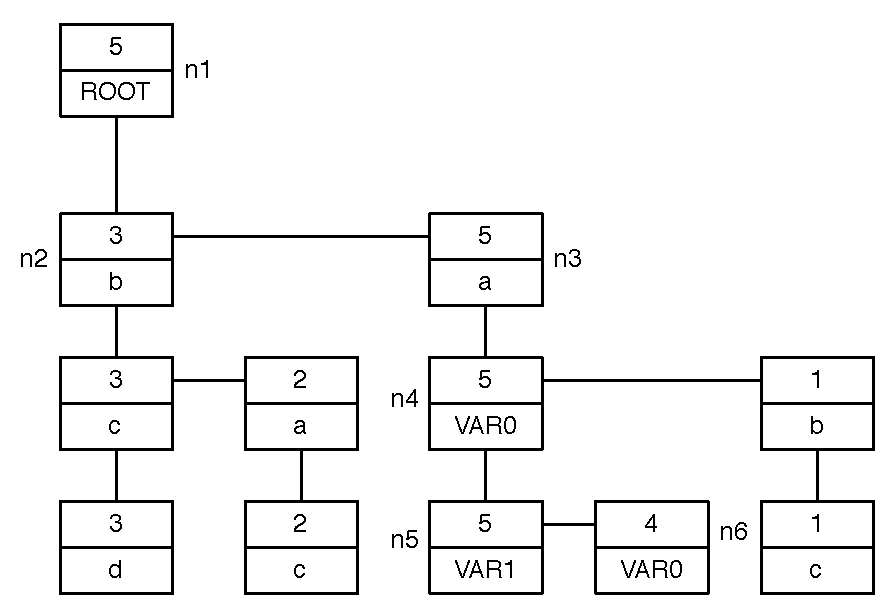
\includegraphics[scale=0.6]{collect_example_1.pdf}}%
   \vspace{40pt}\\
   
   \subfloat[][At trie node $n1$.]{%
      \label{fig:tst_constant_b}%
      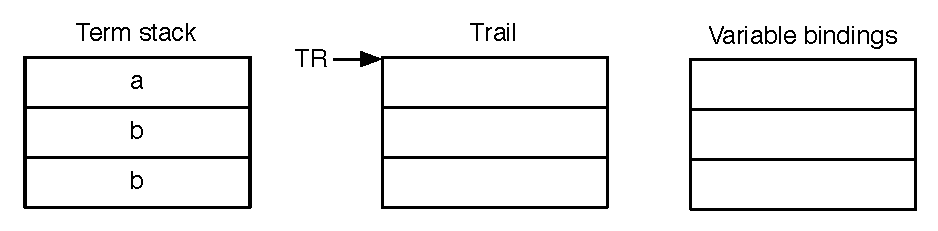
\includegraphics[scale=0.45]{collect_ex1.pdf}}%
   \qquad
   \subfloat[][At trie node $n4$.]{%
      \label{fig:tst_constant_c}%
      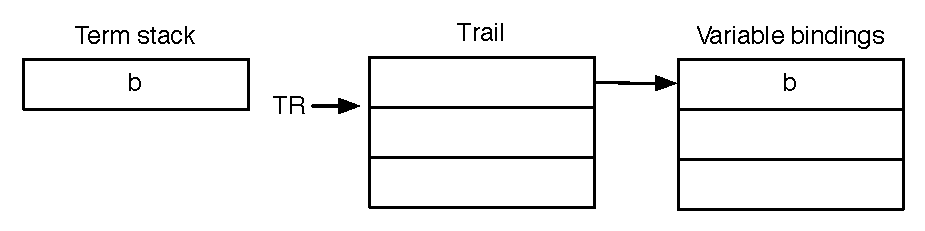
\includegraphics[scale=0.45]{collect_ex2.pdf}} \\
   
   \subfloat[][New answer leaf node $n5$.]{%
      \label{fig:tst_constant_d}%
      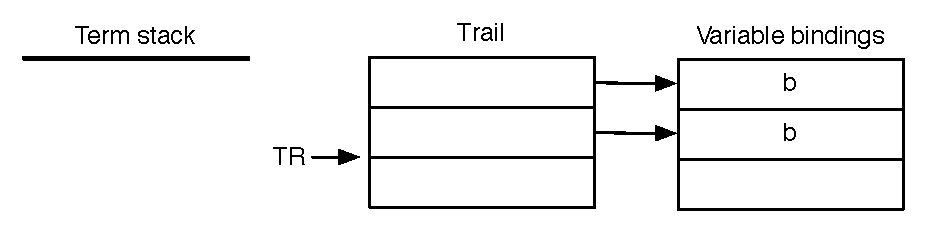
\includegraphics[scale=0.45]{collect_ex3.pdf}}%
   \qquad
   \subfloat[][Backtracking to node $n6$.]{%
      \label{fig:tst_constant_e}%
      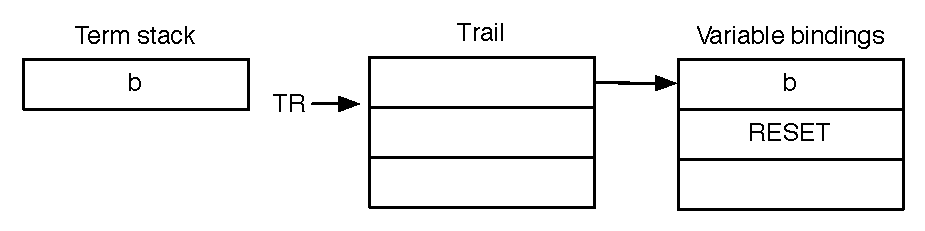
\includegraphics[scale=0.45]{collect_ex4.pdf}} \\
   
   \subfloat[][New answer as the leaf node (f).]{%
      \label{fig:tst_constant_f}%
      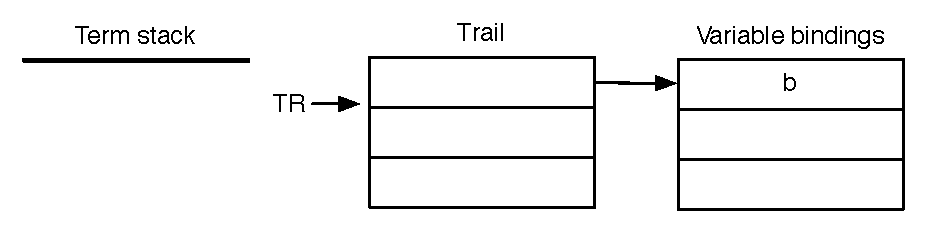
\includegraphics[scale=0.45]{collect_ex5.pdf}}%
   \qquad
   \subfloat[][Untrailing variables and returning.]{%
      \label{fig:tst_constant_g}%
      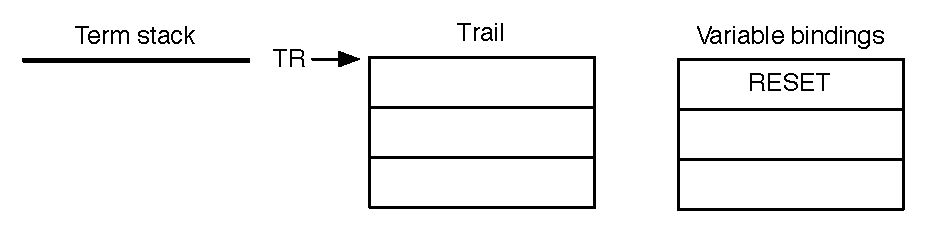
\includegraphics[scale=0.45]{collect_ex6.pdf}} \\
   
   \caption{Unification of answer template \texttt{\{a,~b,~b\}} with time stamp 3.}
   \label{fig:tst_constant}
\end{figure}

We start on node $n1$, the root of the trie (Figure~\ref{fig:tst_constant}). The unify chain
is composed by nodes $n2$ and $n3$. Node $n2$ is discarded because its time stamp is invalid,
but node $n3$ has a valid time stamp and its symbol matches \texttt{a} (Figure~\ref{fig:tst_constant_b}).

On node $n3$, only our first alternative, node $n4$, has a valid time stamp and, after doing
\texttt{trie\_deref} we find an unbound variable, \texttt{VAR0}, which is represented
by the first position of the variable bindings vector.
This variable is trailed and bound to \texttt{b},
resulting in what is presented in Figure~\ref{fig:tst_constant_c}.

On node $n4$, the unify chain is composed by nodes $n5$ and $n6$. Both have valid time stamps ($> 3$).
Node $n5$ is attempted first and easily unifies, because it is an unbound trie variable.
Leaf node $n5$ is our first answer (Figure~\ref{fig:tst_constant_d}).

Now, we need to backtrack to collect more answers. The top choice point frame is retrieved from the
stack resulting in a variable being untrailed and the term \texttt{b} being pushed into the term
stack (Figure~\ref{fig:tst_constant_e}).

In node $n6$ we dereference the trie variable \texttt{VAR0} and get the constant term \texttt{b},
which matches the target term. No binding or trailing is needed and we succeed in collecting another
relevant answer (Figure~\ref{fig:tst_constant_f}).

As there are no more available choice points we need to untrail any bindings made and return
the answers found (Figure~\ref{fig:tst_constant_g}), finishing the search.

\subsection{Unification of Structured Terms}

For structured terms, the unification process is similar to constant unification
(Figure~\ref{fig:unify_structured_term}). First, we check if the current trie node is an
hash table and then the match and unify chains are computed. If the match chain contains
a valid trie node, before we descend into the child node we must push the functor or list
arguments into the term stack, so they can be unified with the next trie nodes.

\begin{figure}[h]
\begin{Verbatim}
unify_structured_term(term, node, ts) {
  if (is_hash_table(node))
    // retrieve the indexed and variable buckets
    (match_chain, unify_chain) = set_match_and_unify_chains(term, node)
    if (match_chain != unify_chain)
      node = search_chain_exact_match(term, match_chain, unify_chain, ts)
      if (node != NULL)
         push_arguments(term_stack, term)
         return node
      // exact match failed
      node = unify_chain
    if (node is NULL)
      return NULL
  return search_chain_unify_with_structured_term(term, node, ts)
}
\end{Verbatim}
\caption{Pseudo-code for procedure \texttt{unify\_structured\_term}.}
\label{fig:unify_structured_term}
\end{figure}

When using the unify chain (procedure \texttt{search\_chain\_unify\_with\_structured\_term}),
we also iterate the chain looking for valid time stamped nodes. For each valid node
four situations may arise (Figure~\ref{fig:search_chain_unify_with_structured_term}):

\begin{enumerate}
  \item The trie symbol is a variable, which is trailed and bound to the structured term;
  \item The trie symbol is a structured term and matches our functor or list.
  The term arguments are pushed into the term stack for unification;
  \item We find a trie variable bound to a structured term. The WAM function \texttt{unify}
  is executed to check for a match and perform additional unifications;
  \item No match was found, the next alternative node is inspected.
\end{enumerate}

\begin{figure}[ht]
\begin{Verbatim}
search_chain_unify_with_structured_term(term, chain, ts) {
  chain = next_valid_node(chain, ts)
  while (chain != NULL)
    alt_chain = next_valid_node(sibling(chain), ts)
    symbol = trie_deref(symbol(chain))
    if (is_variable(symbol)) // case (1)
      push_choice_point_frame(choice_point_stack, alt_chain)
      bind_and_conditionally_trail(symbol, term)
      push(term_log_stack, term)
      return chain
    else if (is_functor(symbol) or is_list(symbol))
      if ((is_functor(symbol(chain)) or is_list(symbol(chain))) and symbol == term)
        // case (2)
        push_choice_point_frame(choice_point_stack, alt_chain)
        push(term_log_stack, term)
        push_arguments(term_stack, term)
        return chain
      else if (unify(term, symbol)) // case (3)
        // trie variable bound to an heap structured term
        push_choice_point_frame(choice_point_stack, alt_chain)
        push(term_log_stack, term)
        return chain
    else
      chain = alt_chain
  }
  // case (4)
  return NULL
}
\end{Verbatim}
\caption{Pseudo-code for procedure \texttt{search\_chain\_unify\_with\_structured\_term}.}
\label{fig:search_chain_unify_with_structured_term}
\end{figure}

Let's consider the time stamped trie in Figure~\ref{fig:tst_functor_a}
and the following answer template: $\{$\texttt{STR 3, STR 6, STR 9}$\}$.
The target time stamp is 1.

\begin{figure}
   \centering
   
   \subfloat[Time stamped trie and heap.]{%
      \label{fig:tst_functor_a}%
      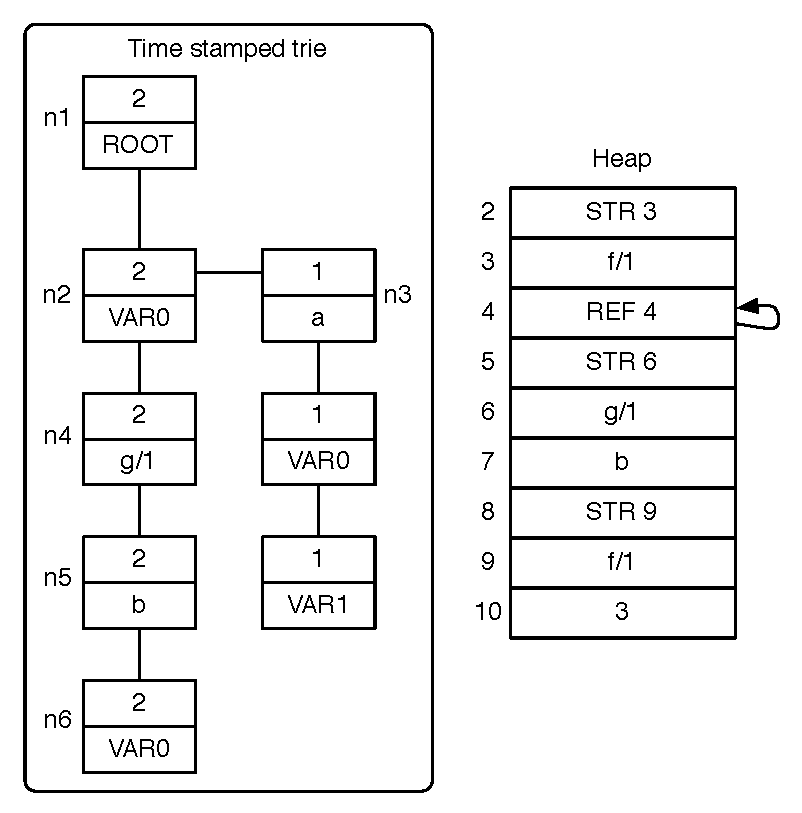
\includegraphics[scale=0.6]{collect_functor.pdf}
   }%
   \vspace{40pt}\\
   
   \subfloat[][At node $n1$.]{%
      \label{fig:tst_functor_b}%
      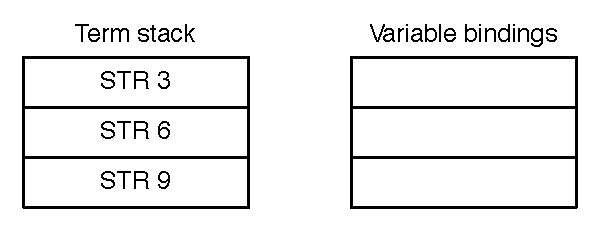
\includegraphics[scale=0.45]{collect_functor1.pdf}}%
   \qquad
   \subfloat[][At node $n2$.]{%
      \label{fig:tst_functor_c}%
      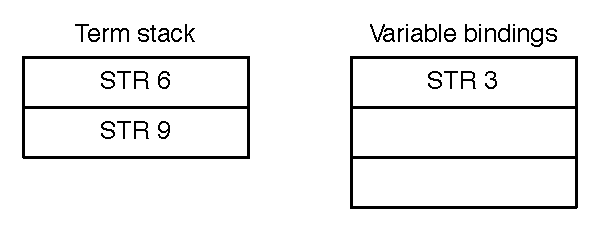
\includegraphics[scale=0.45]{collect_functor2.pdf}} \\
   
   \subfloat[][At node $n4$.]{%
      \label{fig:tst_functor_d}%
      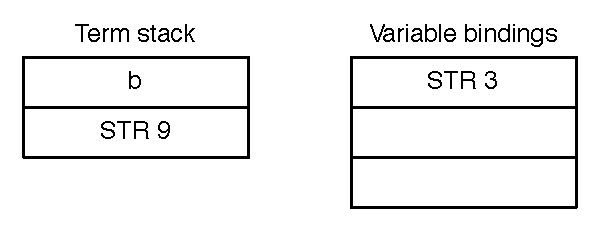
\includegraphics[scale=0.45]{collect_functor3.pdf}}%
   \qquad
   \subfloat[][At node $n5$.]{%
      \label{fig:tst_functor_e}%
      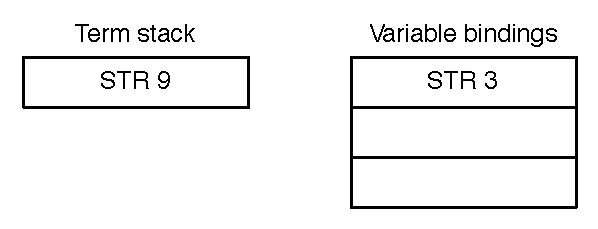
\includegraphics[scale=0.45]{collect_functor4.pdf}} \\
   
   \subfloat[][At node $n6$.]{%
      \label{fig:tst_functor_f}%
      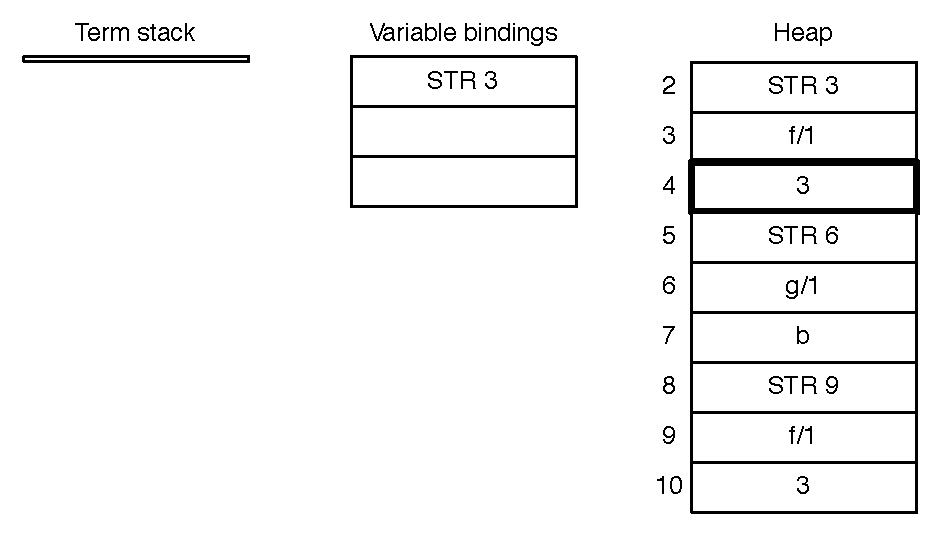
\includegraphics[scale=0.45]{collect_functor5.pdf}} \\
      
   \caption{Unification of answer template \texttt{\{f(X),~g(b),~f(3)\}} with time stamp 1.}
   \label{fig:tst_functor}
\end{figure}

Initially, at node $n1$, the term stack contains the full answer template and the variable bindings vector
is empty (Figure~\ref{fig:tst_functor_b}). Here, only node $n2$ satisfies the time stamp requirements
($2 > 1$).

Node (b) contains a trie variable and the current term is \texttt{STR 3} or \texttt{f(VAR)}.
In this situation, the variable bindings position for \textbf{VAR0} is trailed and bound to \texttt{STR 3}
(Figure~\ref{fig:tst_functor_c}).

Next, node $n4$ contains the symbol \texttt{g/1} and the current term is \texttt{STR 6}
or \texttt{g(b)}, which matches. The argument \texttt{b} of \texttt{g(b)}
is thus pushed into the term stack to be processed in the next node (Figure~\ref{fig:tst_functor_d}).

Then, node $n5$ has the symbol \texttt{b}, which matches with \texttt{b} from the term stack, and
execution proceeds to node $n6$ (Figure~\ref{fig:tst_functor_e}).

At $n6$ we find a trie variable, which, after being dereferenced, contains the
functor \texttt{f(VAR)}. The current term to be unified is \texttt{f(3)}.
In this situation we call \texttt{unify}, which will try to unify both terms.
The unification has the side effect of setting the heap variable cell 4 to \texttt{3}
(Figure~\ref{fig:tst_functor_f}).
This variable is conditional because it is positioned before the register \texttt{HB},
which given the algorithm must be greater than 10.

\subsection{Unification of Variable Terms}

Variable unification is done when the next term to unify is a variable. In this case, trie branches are only pruned
by using the time stamp as variables can unify with anything.
Figure~\ref{fig:unify_variable_term} presents the procedure \texttt{unify\_variable\_term}. In this function, three
situations may arise:

\begin{enumerate}
  \item The current node is an hash table. In this situation we can select the next transitions
   by using the time stamped index, which can efficiently prune based on the time stamp. Notice that we visit
   an hash table only once, subsequent backtracking uses the time stamp index nodes;
  \item The current node is inside an hash table and thus indexed on the time stamp index.
   The node is matched against the variable and the alternative node is selected by following
   the index chain link;
  \item Current node is a simple sibling chain. Both the chain and the alternative chain are set by
   iterating over the node chain, looking for valid time stamps.
\end{enumerate}

\begin{figure}[h]
\begin{Verbatim}
unify_variable_term(variable, node, ts) {
  if (is_hash_table(node))
     // case 1: current node is an hash table
    index = index_head(node)
    if (timestamp(index) > ts)
      node = node(index)
      alt_chain = node(next_valid_index_node(index, ts))
    else
      return NULL
  else if (is_hashed_node(node))
    // case 2: current node is an hashed node and has a corresponding index node
    // can only be here via backtracking
    alt_chain = node(next_valid_index_node(index_node(node), ts))
  else
    // case 3: simple chain of siblings
    node = chain_next_valid_node(node, ts)
    if (node == NULL)
      return NULL
    alt_chain = sibling(node)
  
  push_choice_point_frame(choice_point_stack, alt_chain)
  push(term_log_stack, variable)
  symbol = trie_deref(symbol(node))
  return unify_with_variable(variable, symbol, node)
}
\end{Verbatim}
\caption{Pseudo-code for procedure \texttt{unify\_variable\_term}.}
\label{fig:unify_variable_term}
\end{figure}

Once the chains are set, we create a new choice point, run the variable unification algorithm
and proceed into the next trie node.
From the pseudo-code in Figure~\ref{fig:unify_with_variable}, unification with a term variable
is dictated by the type of trie symbol. It follows the following rules:

\begin{itemize}
  \item Constant: the term variable is bound to the symbol and conditionally trailed;
  \item Structured term: if the symbol was a trie variable bound to a term then we bind
  the variable to the heap location; else, we create a new structure (functor or list) on the heap and bind
  the variable to it, resulting in a term with various heap variables as arguments, which will be pushed into
  the term stack and will be used in the next iterations of the algorithm;
  \item Variable: if the variable is a trie variable, we bind and trail it; if it is an heap variable that
  was dereferenced from a trie variable using \texttt{trie\_deref}, \texttt{unify} chooses the binding direction,
  resulting in one of the variables being trailed.
\end{itemize}


\begin{figure}[ht]
\begin{Verbatim}
unify_with_variable(variable, symbol, node) {
  if (is_constant(symbol))
    bind_and_conditionally_trail(variable, symbol)
  else if (is_functor(symbol) or is_list(symbol))
    if (is_list(symbol(node)) or is_functor(symbol(node))
      term = create_heap_structure(symbol)
      bind_and_conditionally_trail(variable, term)
      // push new structure arguments
      push_arguments(term_stack, deref(variable))
    else
      // trie variable bound to an heap structure
      bind_and_conditionally_trail(variable, symbol)
  else if (is_variable(symbol))
    if (is_trie_variable(symbol))
      bind_and_trail(symbol, variable)
    else
      // two heap variables
      unify(symbol, variable)
  else
    return NULL
  
  return node
}
\end{Verbatim}
\caption{Pseudo-code for procedure \texttt{unify\_with\_variable}.}
\label{fig:unify_with_variable}
\end{figure}

As an example, consider the trie and heap in Figure~\ref{fig:tst_variable_a}.
The input answer template is \texttt{\{REF~2,REF~2,~b\}} and the target time stamp is 2.

\begin{figure}
   \centering
   
   \subfloat[Time stamped trie and heap.]{%
      \label{fig:tst_variable_a}%
      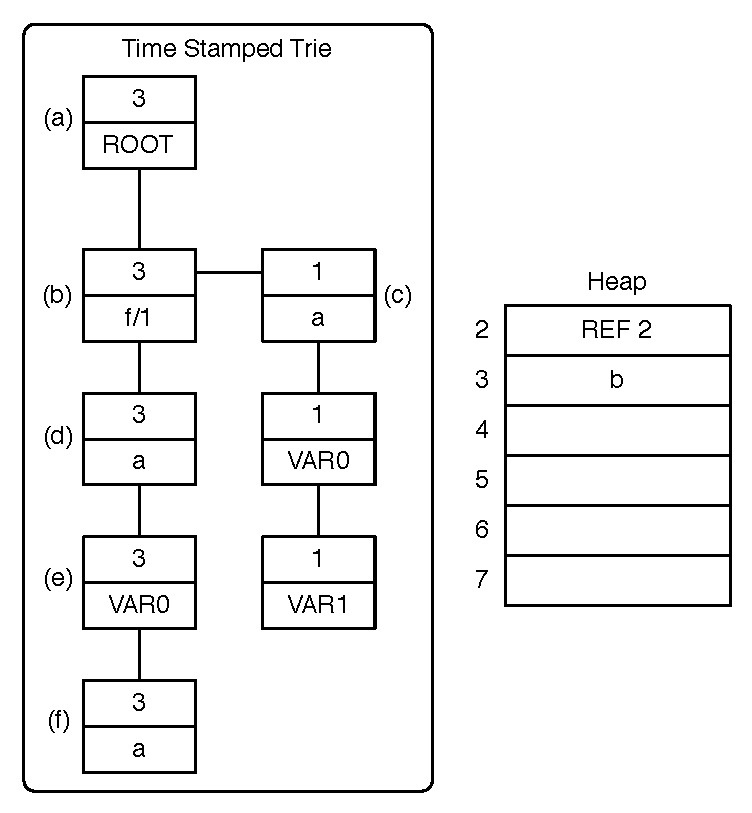
\includegraphics[scale=0.6]{collect_variable.pdf}
   }%
   \vspace{40pt}\\
   
   \subfloat[][At node $n1$.]{%
      \label{fig:tst_variable_b}%
      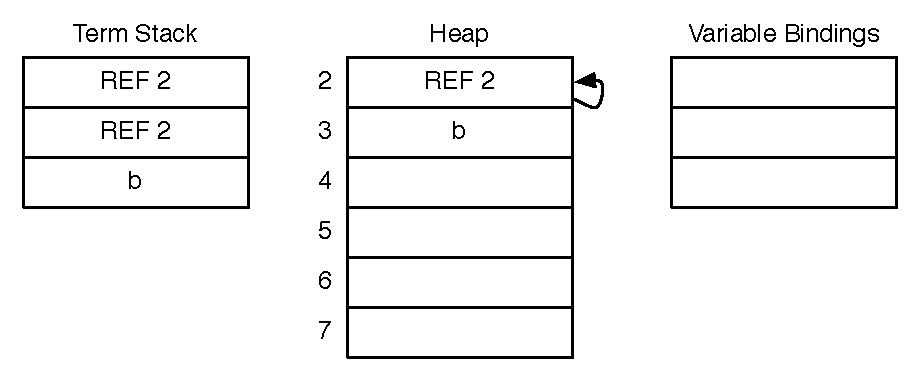
\includegraphics[scale=0.45]{collect_variable1.pdf}}%
   \qquad
   \subfloat[][After unifying with node $n2$.]{%
      \label{fig:tst_variable_c}%
      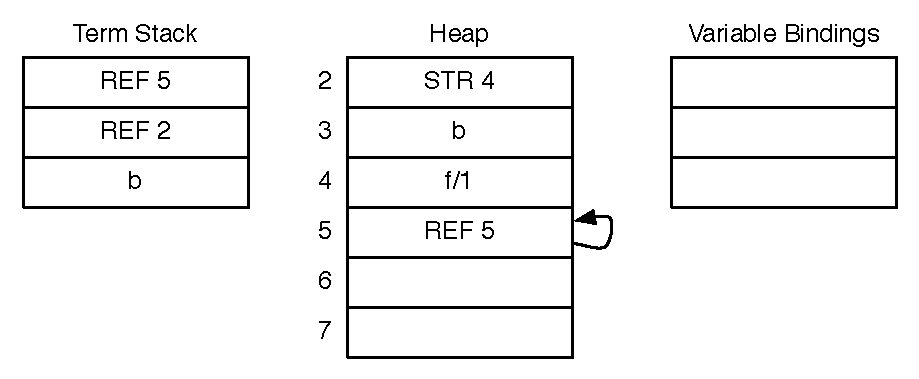
\includegraphics[scale=0.45]{collect_variable2.pdf}} \\
   
   \subfloat[][After unifying with node $n4$.]{%
      \label{fig:tst_variable_d}%
      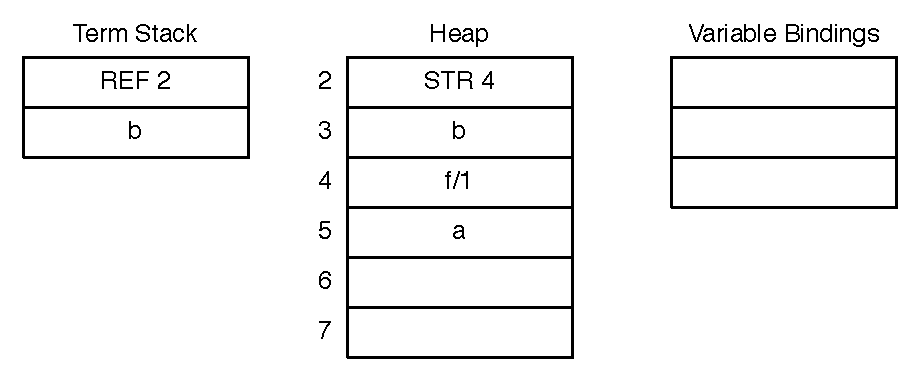
\includegraphics[scale=0.45]{collect_variable3.pdf}}%
   \qquad
   \subfloat[][After unifying with node (e).]{%
      \label{fig:tst_variable_e}%
      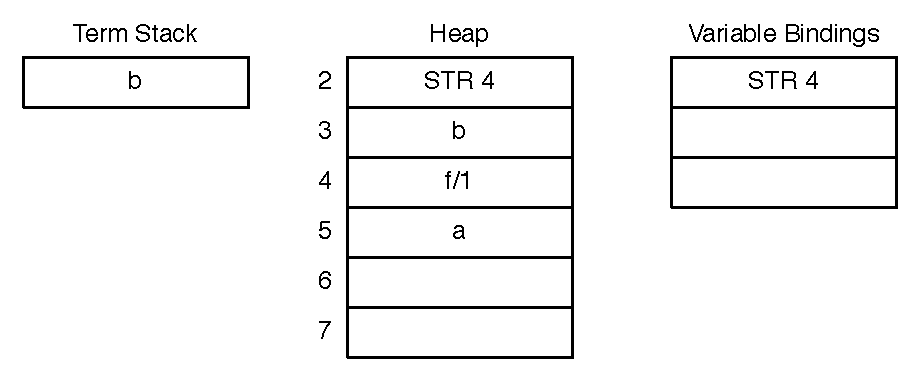
\includegraphics[scale=0.45]{collect_variable4.pdf}} \\
   
   \caption{Unification of answer template \texttt{\{REF~2,REF~2,~b\}} with time stamp 2.}
   \label{fig:tst_variable}
\end{figure}

On root node $n1$, we start with the configuration presented in Figure~\ref{fig:tst_variable_b}.

Node $n2$ is then the only valid transition, with time stamp 3.
The functor \texttt{f/1} is unified against the variable \texttt{REF 2},
which results in the functor \texttt{f/1} being created on the heap
and its argument (\texttt{REF 5}) being pushed into the term stack
(Figure~\ref{fig:tst_variable_c}).

The yet unbound functor argument matches atom \texttt{a} in node $n4$,
resulting in the update of the heap cell 5 (Figure~\ref{fig:tst_variable_d}).

Now on the term stack we have \texttt{REF 2}, which dereferences to
a structure on cell 4, and on node $n5$ we have the unbound trie variable
\texttt{VAR0}, that gets bound to \texttt{STR 4} (Figure~\ref{fig:tst_variable_e}).

Finally, the last term on the term stack is \texttt{b}, which
can not be matched against \texttt{a} on node $n6$, hence no
relevant answers are found on this trie.

\section{Consuming Answers}

Each consumer subgoal frame stores a linked list with all the answers collected
during evaluation. This list is built incrementally and
whenever a consumer choice point exhausts its answer list, the retrieval
of new relevant answers is attempted in order to reflect the answers generated in the meantime
by the generator subgoal.

While the retrieval of relevant answers is done in one step by searching the answer trie
and pruning branches by time stamp and unification failure, the consumption of
answers is done by consuming one answer at a time and is completely separated from the collection phase.

Consider an answer $A$ with a trie path from a leaf node $L$ to
the trie root $R$. Consuming $A$ amounts to unifying the symbols on the trie path
to the answer template $AT$ that was built for the consumer choice point. In such a way that, in the end,
the variables on $AT$ match the answer on the trie.

As we are certain that $A$ unifies with $AT$, consumption is reduced to a simple unification
between $AT$ and the trie nodes from $L$ to $R$.
Implementation wise, we use the term stack that is initially pushed with $AT$
and a symbol stack containing symbols from $L$ to $R$. Then, we proceed by
iteratively popping one term from the term stack and one symbol from the symbol stack
and unifying one against the other.

In Figure~\ref{fig:consume_answer}, we present an example showing the data structures involved in consuming
a subsumptive answer. The subsumptive subgoal is \texttt{p(X,Y,Z)} and the
subsumed subgoal is \texttt{p(d,f(X),3)}. The answer to consume is \texttt{p(d,f(a),3)},
which corresponds to the binding \texttt{\{X~=~a\}}.

\begin{figure}[h]
  \centering
    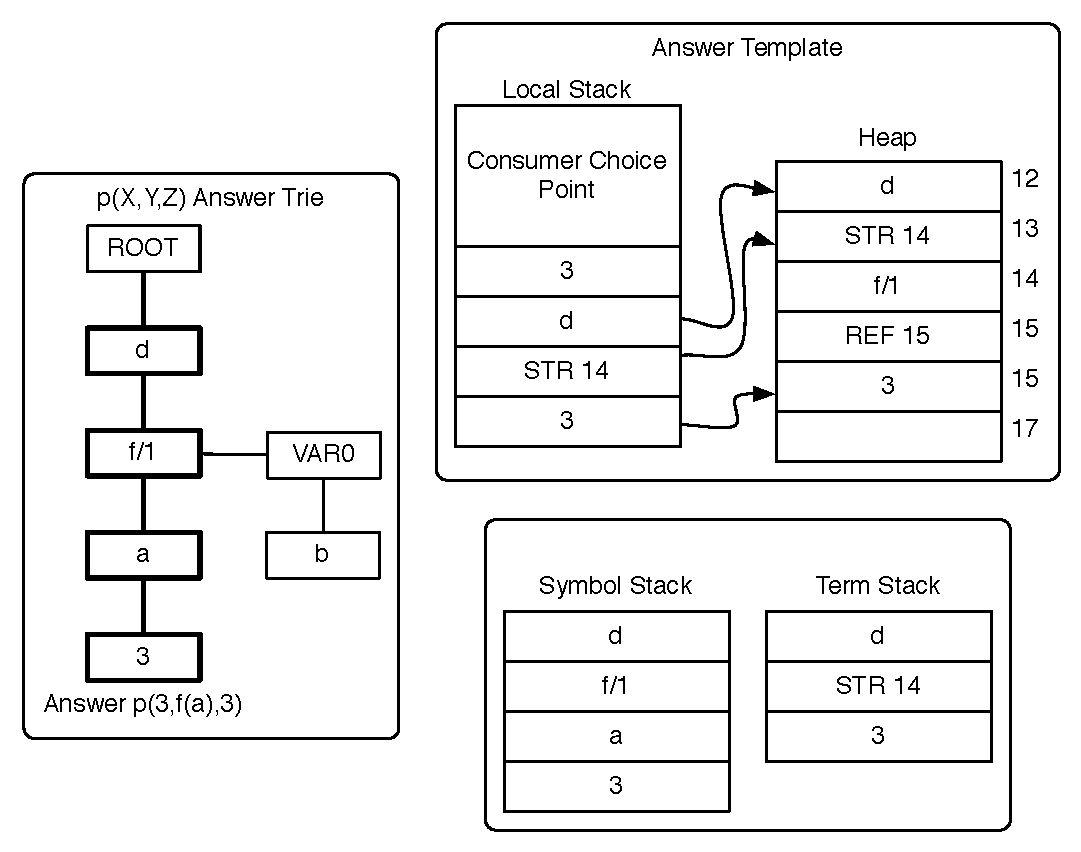
\includegraphics[scale=0.40]{consume_answer.pdf}
  \caption{Data structures related to answer consumption.}
  \label{fig:consume_answer}
\end{figure}

\section{Compiled Tries}\label{sec:compiled_tries}

After an answer trie is completed, we can optimize the process of consuming answers from a complete
subgoal by annotating each trie node with a \textit{trie instruction}. This optimization technique
is called \textit{compiled tries} \cite{RamakrishnanIV-99}.

Compiled tries are based on the observation that all common prefixes of the terms in a trie
are shared during execution of trie instructions. Thus, when backtracking
through the terms of a trie, each transition is taken at most only once.

In Figure~\ref{fig:compiled_trie}, we represent a compiled answer trie for the subgoal
\texttt{p(X,Y,Z)}. Notice that each node is extended with an instruction field.
The instruction set follows the standard WAM instruction style with \textit{try},
\textit{retry} and \textit{trust}. On a sibling chain the leftmost nodes are marked
with \textit{try} instructions and middle nodes with \textit{retry} instructions. Rightmost
nodes use \textit{trust} instructions, while single nodes use \textit{do} instructions.

\begin{figure}[h]
  \centering
    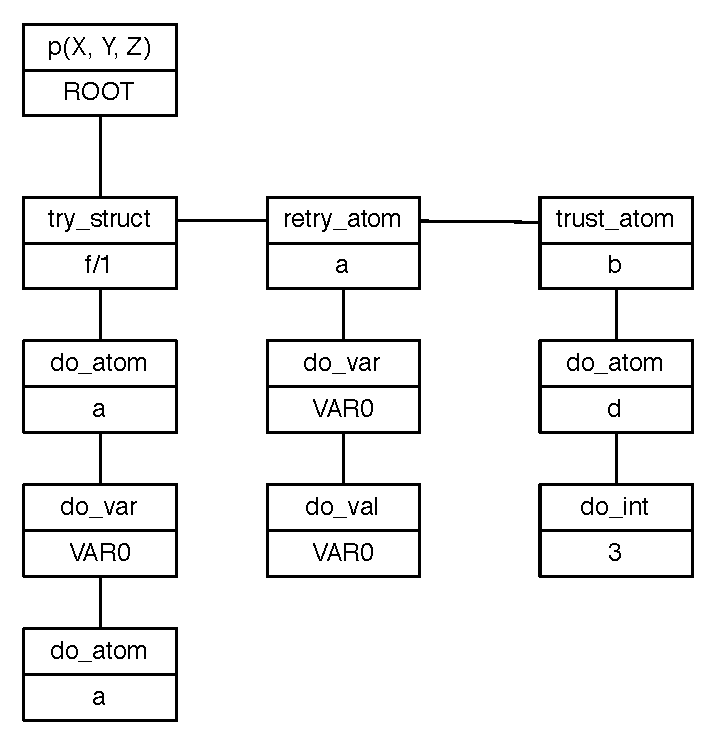
\includegraphics[scale=0.6]{compiled_trie.pdf}
  \caption{A compiled trie for subgoal \texttt{p(X,Y,Z)}.}
  \label{fig:compiled_trie}
\end{figure}

A \textit{try} instruction creates a new WAM choice point pointing to the sibling node,
while \textit{retry} instructions change the previous choice point to point to the next sibling node,
thus enabling us to navigate to new trie branches while backtracking. The \textit{trust}
instruction removes the choice point as no more siblings are available. Finally, \textit{do}
instructions do not create choice points as no backtracking options are available.

In a variant tabling engine, each trie instruction just binds each variable on the substitution factor to a term.
On structured terms, like functors or lists, the term is first built on the heap and then
bound to the current variable, while the unbound arguments are then passed into the next trie levels
to be instantiated.

In XSB, time stamped tries are used to evaluate subsumed subgoals while the subsuming subgoal
is incomplete, thus providing incremental retrieving of answers.
When a subgoal $G$ completes, the engine uses the compiled answer trie from $G$
to evaluate a subsumed subgoal $G'$, instead of loading each individual answer.
Not all answers of from $G$ will be relevant to $G'$, thus we must prune irrelevant paths
through the process of unification. 

Some modifications are thus required to use compiled tries in subsumptive tabling. First,
instead of using the substitution factor when running compiled code, we use the answer template.
Next, each instruction must now do unifications instead of simple bind operations,
because in addition to unbound variables, these instructions can also receive instantiated terms.
Finally, while each instruction succeeds when running with the substitution factor of the generator
subgoal, for subsumed subgoals some instructions can fail, because not every answer will be relevant,
hence will not unify with the answer template. The unification operations applied on each trie node
are similar to the unifications done while collecting relevant answers in time stamped tries
(Section \ref{sec:collect}).

Variant engines like YapTab collapse each hash table into a chain of nodes before compiling
the trie. While this technique makes sense for a variant engine, in subsumptive engines
having hash tables helps the unification process by enabling fast search of instantiated terms.
If we had a very long sibling chain, locating a specific term would have a linear time complexity, while
hash tables provide $O(1)$ search complexity.
Thus, instead of removing hash tables, they must be kept on a subsumptive tabling engine.
To use the hash tables, we must extend the trie instruction set with a new instruction,
\textit{do\_hash} (Figure~\ref{fig:compiled_hash}).

\begin{figure}[h]
  \centering
    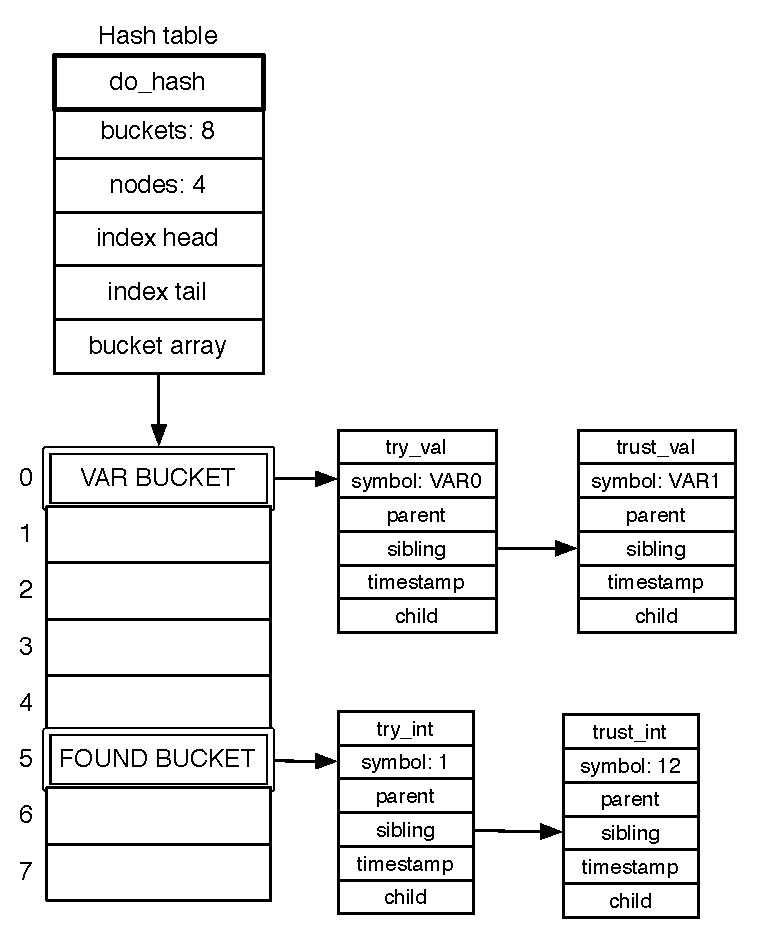
\includegraphics[scale=0.6]{compiled_hash.pdf}
  \caption{Compiled hash table.}
  \label{fig:compiled_hash}
\end{figure}

When the next term to unify is instantiated, we first lookup the bucket for this
term and execute the code of the bucket chain. But periodically, we store a choice point that will
execute code from the variable bucket, because variables can unify with any term.

If the term is a variable, we must visit every trie node in the hash table. This is done
by storing a choice point that keeps the next hash bucket to be executed.

\section{Call Subsumption in YapTab}

Our first attempt to extend the variant YapTab engine to support call by subsumption
involved importing the subsumption related algorithms and data structures described in
the previous sections from XSB into YapTab. These algorithms were imported as faithful as possible,
hence very little modifications were made as C macros were used to translate the original
code to YapTab. Sections of code specific to XSB or Yap were protected with conditional
compilation, thus enabling both Prolog systems to use the same code.

In this section we will describe in more detail the modifications made to the following components of YapTab:
tabled data structures, tabling operations and compiled tries.
This new version of YapTab is called \textit{YapTab\_TST} and will be described in the next sections.

\subsection{Data Structures}

This section describes the modifications and extensions made to existent data structures
in order to implement \textit{YapTab\_TST}.

\subsubsection{Table Entry}

Each table entry contains a bit field called \textbf{mode\_flags} which stores information about
the behavior of the corresponding tabled predicate. The original YapTab supports the
following mutually exclusive flags: \textbf{batched} / \textbf{local}, for defining the scheduling strategy;
and \textbf{load answers} / \textbf{exec answers}, the later makes the engine to use compiled tries,
while the first forces the engine to load a completed table by loading answers individually.

Two new mutually exclusive flags were created for \textit{YapTab\_TST}: \textbf{variant},
which forces the predicate to use variant tabling and \textbf{subsumptive} to use subsumptive tabling.

\subsubsection{Trie Nodes}

YapTab uses two types of trie nodes: subgoal trie nodes, for subgoal tries; and answer trie nodes, for
answer tries. In terms of hash tables, the same data structures are used for both subgoal and answer
hash tables. \textit{YapTab\_TST} extends the answer and subgoal trie nodes with a \textbf{status}
bit field and implements the time stamped trie nodes as answer trie nodes extended with a \textbf{timestamp} field.
The \textbf{status} bit field is used to identify the type of trie node, i.e., if it is
an hash table, a leaf node or an hashed node.
For hash tables, we extended the answer hash table with the time stamp indexes to create the
time stamped hash table. The index data structure was integrally copied from XSB.

\subsubsection{Subgoal Frames}

The subgoal frame structure in YapTab is a main component of the table space.
It contains the fields: \textbf{answer\_trie}, a pointer to the answer trie;
\textbf{state}, the state flag; \textbf{first\_answer} and \textbf{last\_answer},
as the answer return list; \textbf{next}, a pointer to the next executing subgoal;
and \textbf{generator\_cp}, which points to the generator choice point.

Two new kinds of subgoal frame were created: the \textit{subsumptive generator subgoal frame} and
the \textit{subsumed consumer subgoal frame}.

The subsumptive generator subgoal frame extends the original variant subgoal frame
with the field \textbf{consumers}. This field points to a consumer subgoal frame and works
as a chain link to the subsumed subgoal frames of the generator subgoal.

The subsumptive consumer subgoal frame does not extend the variant subgoal frame, because
some variant fields are not needed.
The consumer frame contains the following fields: \textbf{state}, the state of execution;
\textbf{generator}, a pointer to the subsumptive generator subgoal frame; \textbf{consumer\_cp},
a pointer to the first consumer choice point; \textbf{first\_answer} and \textbf{last\_answer},
as the answer return list; \textbf{ts}, the consumer time stamp;
\textbf{next}, a pointer to the next evaluating consumer subgoal frame; \textbf{answer\_template},
a pointer to the answer template built on the heap; and \textbf{consumers},
to link consumer subgoals of the generator subgoal frame.

Each subgoal frame was also extended with a \textbf{type} field, which identifies the subgoal frame type.
The variant subgoal frame now uses an answer return list instead of using the \textbf{child} field of
each trie node to link answers.

Figure~\ref{fig:subgoal_frames} illustrates a subgoal trie for the predicate \texttt{p/2}
with the following subgoals: \texttt{p(X,Y)}, as a generator subgoal; and \texttt{p(2,X)} and
\texttt{p(3,X)} as consumer subgoals.

\begin{figure}[h]
  \centering
    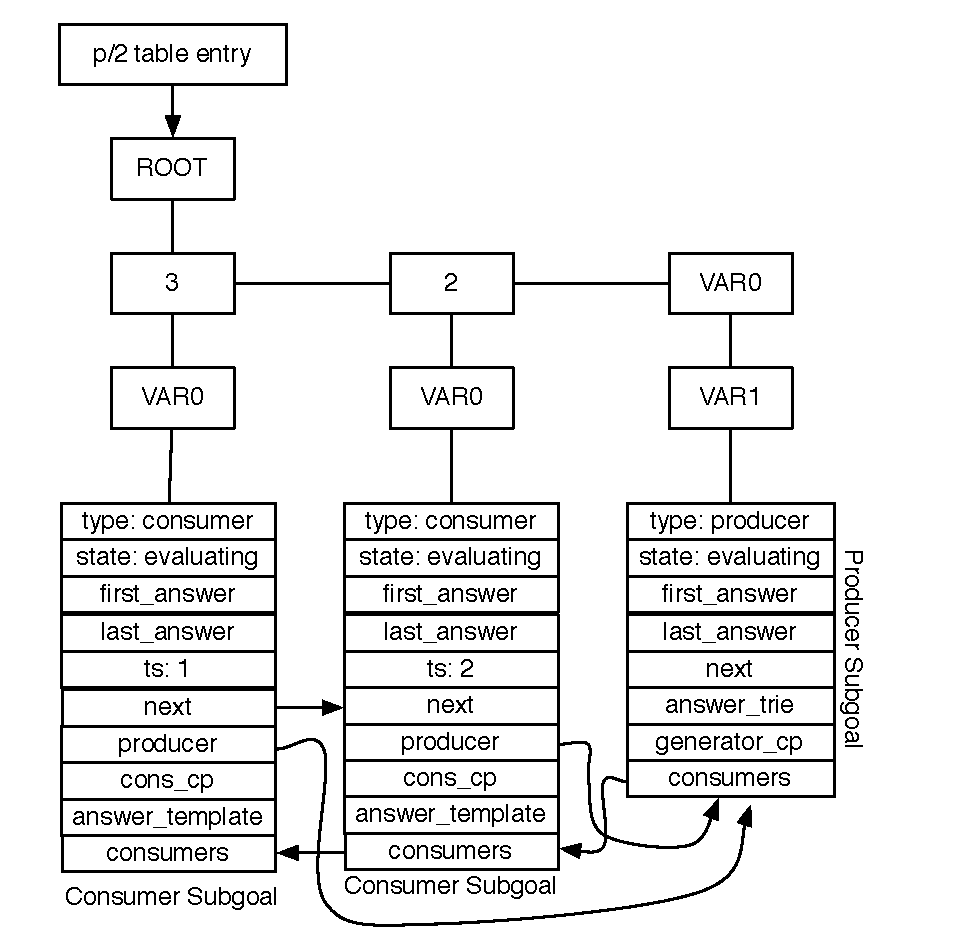
\includegraphics[scale=0.6]{subgoal_frames.pdf}
  \caption{Subgoal trie with a subsumptive generator and two subsumed consumer subgoal frames.}
  \label{fig:subgoal_frames}
\end{figure}

\subsection{Tabled Subgoal Call}

The tabled subgoal call operation is one of the four main tabling operations. In YapTab,
if a subgoal call is already on the table space, a new consumer node is allocated and
the execution runs the answer resolution operation, in order to consume answers.
Otherwise, a new generator node is allocated and the subgoal compiled code is executed.

Figure~\ref{fig:tabled_subgoal_call} presents the pseudo-code for the original tabled subgoal call operation.
In the consumer case, we use the \texttt{find\_dependency\_node} and \texttt{find\_leader\_node} procedures
to locate the leader node for this consumer. The function \texttt{find\_dependency\_node} simply
returns the choice point of the generator node for this subgoal, while \texttt{find\_leader\_node}
iterates the dependency space between \texttt{dependency} and the new dependency frame for this consumer,
to locate a dependency frame in which the leader is outside this range. If no such dependency frame
exists, the leader node is set as the generator choice point found in \texttt{find\_dependency\_node},
else we use the leader of the dependency frame that satisfied the previous condition. \cite{Rocha-PhD}

\begin{figure}[ht]
\begin{Verbatim}
tabled_subgoal_call(table_entry, arguments) {
  subgoal_frame = subgoal_search(subgoal_trie(table_entry), arguments)
  
  if (state(subgoal_frame) == READY)
    // new generator
    store_generator_node(table_entry, arguments, subgoal_frame)
    jump_to_predicate_code()
  else if (state(subgoal_frame) == EVALUATING)
    // new consumer
    dependency = find_dependency_node(subgoal_frame)
    leader = find_leader_node(subgoal_frame, dependency)
    store_consumer_node(table_entry, subgoal_frame, leader)
    jump_to_answer_resolution()
  else
    // subgoal is completed
    if (state(answer_trie(subgoal_frame)) != COMPILED)
      compile_answer_trie(answer_trie(subgoal_frame))
    execute_answer_trie(answer_trie(subgoal_frame))
}
\end{Verbatim}
\caption{Pseudo-code for the original tabled subgoal call operation.}
\label{fig:tabled_subgoal_call}
\end{figure}

\textit{YapTab\_TST} extends the tabled subgoal call operation to deal with either subsumptive and variant subgoals,
and if a predicate uses call by subsumption, we call the \texttt{subsumptive\_subgoal\_search} procedure
(Figure~\ref{fig:subsumptive_subgoal_search}) to look on the subgoal trie for subsuming subgoals.
If no subsuming path is found, we insert the subgoal path on the subgoal trie and create a new generator
subgoal frame. If some path is found and the subgoal frame is a generator it can be either
a variant of our subgoal or a more general subgoal. For both cases
we use \texttt{construct\_answer\_template\_from\_lookup}, which constructs the right answer template for us.
If the found subgoal frame is a consumer, we must consume from its generator and reconstruct the answer
template by using the generator trie path.
Consumer trie paths are only constructed when the generator subgoal frame is still evaluating.
When the generator is completed, we just execute the compiled trie, so there is no need
to create a consumer subgoal frame.

\begin{figure}[ht]
\begin{Verbatim}
subsumptive_subgoal_search(table_entry, arguments) {
  (path, leaf) = lookup_subsuming_call(subgoal_trie(table_entry), arguments)
  
  if (path == NO_PATH)
    leaf = insert_with_variant_continuation(subgoal_trie)
    local_stack = construct_answer_template_from_insertion(local_stack)
    return create_generator_subgoal_frame(leaf)
  else
    found_sf = subgoal_frame(leaf)
    
    if (type(found_sf) == SUBSUMPTIVE_GENERATOR)
      subsumer_sf = found_sf
      local_stack = construct_answer_template_from_lookup(local_stack)
    else
      subsumer_sf = generator(found_sf)
      local_stack = construct_answer_template_from_generator(subsumer_sf, local_stack)
    
    if (path_type == VARIANT_PATH)
      return found_sf
    
    // subsumptive path
    if (state(subsumer_sf) == EVALUATING)
      // create variant path
      leaf = insert_with_variant_continuation(subgoal_trie)
      copy_answer_template_to_heap(local_stack)
      return create_consumer_subgoal_frame(leaf, subsumer_sf)
    else
      return subsumer_sf
}
\end{Verbatim}
\caption{Pseudo-code for procedure \texttt{subsumptive\_subgoal\_search}.}
\label{fig:subsumptive_subgoal_search}
\end{figure}

When a consumer subgoal frame is created we make a \textit{structural copy} of the answer template
into the heap. A structural copy is made by recursively copying structured terms (functors and lists)
and by making integral copies of constant terms.
For variables, we create a new variable on the heap for each variable on the local stack, in such a way
that no references exist between the two answer templates.
Figure~\ref{fig:structural_copy} illustrates a structural copy of the answer template
\texttt{\{X,~f(a)\}} between the local stack and the heap.

The answer template on the heap will be used as an argument
to the algorithm that collects relevant answers from the generator answer trie.
Each consumer subgoal frame has just one copy of the answer template on the heap,
while each consumer node uses its own answer template built on the local stack to
consume answers, because it references variables
and terms from the arguments.

\begin{figure}[H]
  \centering
    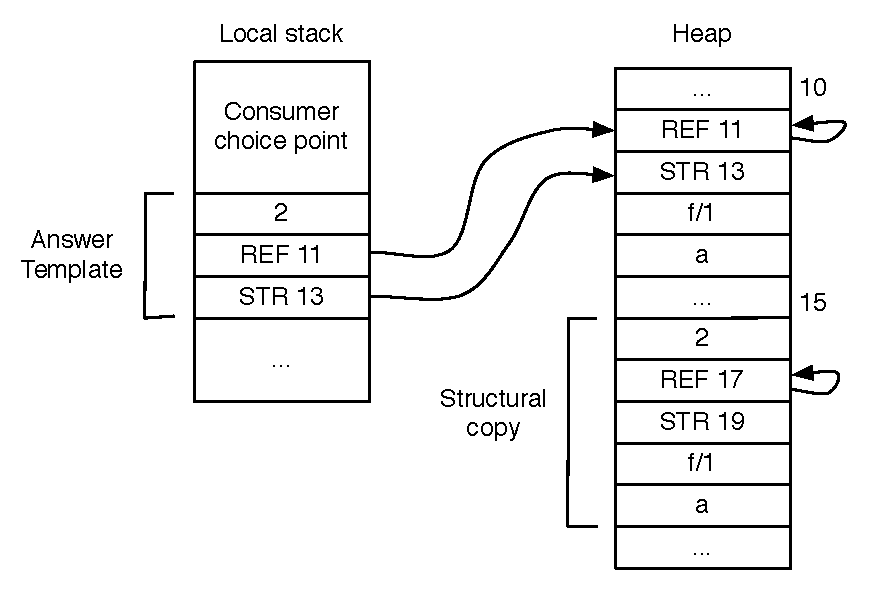
\includegraphics[scale=0.6]{structural_copy.pdf}
  \caption{Making a structural copy of the answer template \texttt{\{X,~f(a)\}}.}
  \label{fig:structural_copy}
\end{figure}

The field \textbf{consumer\_cp} of the consumer subgoal frame is set to point to the first call
of the consumer subgoal and will be used to access the value of \texttt{H} stored on the choice point.
This value of \texttt{H} points to the top of the heap during the choice point creation which corresponds
to the answer template copied before. The field \textbf{answer\_template} points to \texttt{H}
and is used to avoid accessing the choice point, thus it must be recalculated during garbage collection.

This differs from XSB \cite{Johnson-00} where a \textit{non-structural copy} of the answer template
is built on the heap for each consumer node. A non-structural copy is made by making references from
the heap to the terms on the heap. Figure~\ref{fig:non_structural_copy} illustrates a non-structural
copy of the answer template \texttt{\{X,~f(a)\}}. 
while making non-structural copies is faster than doing structural copies, collecting relevant answers
can, potentially, involve more environment switching, because we must reconstitute the environment of
the consumer to ensure that the answer template is valid, which involves using the trail to unbind
and/or rebind variables. Our approach has the disadvantage of making structural copies, but only one
copy is done and there is no need to invoke the algorithm within the environment of the subsumed call.

\begin{figure}[H]
  \centering
    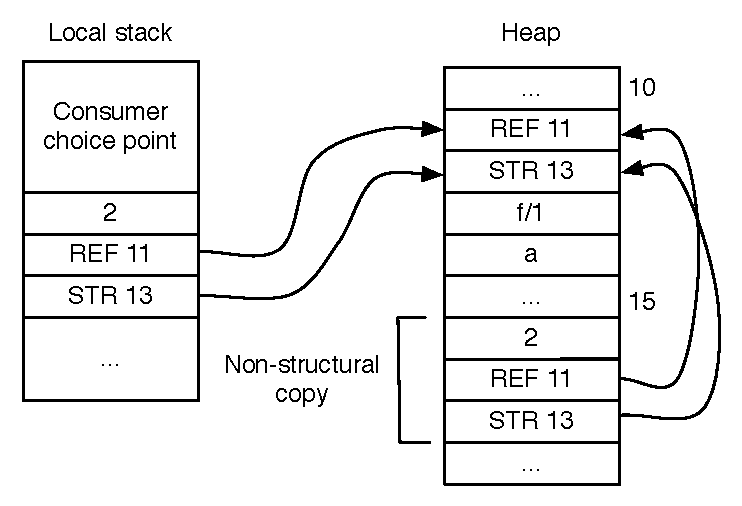
\includegraphics[scale=0.6]{non_structural_copy.pdf}
  \caption{Making a non-structural copy of the answer template \texttt{\{X,~f(a)\}}.}
  \label{fig:non_structural_copy}
\end{figure}

Other modifications were applied to the tabled call operation in order to abstract some details about
variant and subsumptive tabling. Figure~\ref{fig:tabled_subgoal_call_new} shows the updated tabled
subgoal operation.

\begin{figure}[ht]
\begin{Verbatim}
tabled_subgoal_call(table_entry, arguments) {
  subgoal_trie = subgoal_trie(table_entry)
  
  if(mode_flag(table_entry) == VARIANT)
    subgoal_frame = variant_subgoal_search(subgoal_trie, arguments)
  else
    subgoal_frame = subsumptive_subgoal_search(subgoal_trie, arguments)
  
  if (is_new_generator_call(subgoal_frame))                 // CHANGED
    store_generator_node(table_entry, arguments, subgoal_frame)
    jump_to_predicate_code()
  else if (is_new_consumer_call(subgoal_frame))             // CHANGED
    dependency = find_dependency_node(subgoal_frame)
    leader = find_leader_node(subgoal_frame, dependency)
    store_consumer_node(table_entry, subgoal_frame, leader)
                                                            // NEW
    if ((type(subgoal_frame) == SUBSUMED_CONSUMER) and (state(subgoal_frame) == READY))
      recompute_answer_template(subgoal_frame)
      consumer_cp(subgoal_frame) = B
      add_to_consumer_stack(subgoal_frame)
    jump_to_answer_resolution()
  else
    // subgoal is completed
    if (state(answer_trie(subgoal_frame)) != COMPILED)
      compile_answer_trie(answer_trie(subgoal_frame))
    execute_answer_trie(answer_trie(subgoal_frame))
}
\end{Verbatim}
\caption{Pseudo-code for the new tabled subgoal call operation.}
\label{fig:tabled_subgoal_call_new}
\end{figure}

The function \texttt{is\_new\_generator\_call} (Figure~\ref{fig:is_new_generator_call}) inspects the found
subgoal frame in order to tell if a new generator node must be allocated.
For call by subsumption, a new generator is allocated whenever a variant subgoal is not found
on the trie and the resulting subgoal frame is a generator.

\begin{figure}[ht]
\begin{Verbatim}
is_new_generator_call(subgoal_frame) {
  if (type(subgoal_frame) == VARIANT or type(subgoal_frame) == SUBSUMPTIVE_GENERATOR)
    // must be a first call to either a variant or subsumptive generator subgoal
    return state(subgoal_frame) == READY
    
  // consumer subgoal are not generator calls
  return FALSE
}
\end{Verbatim}
\caption{Pseudo-code for function \texttt{is\_new\_generator\_call}.}
\label{fig:is_new_generator_call}
\end{figure}

The function \texttt{is\_new\_consumer\_call} (Figure~\ref{fig:is_new_consumer_call}) decides
that a consumer node must be allocated when:

\begin{enumerate}
  \item The subgoal frame is variant or generator and is currently being evaluated;
  \item Or, the subgoal frame is consumer and the generator subgoal is still evaluating.
\end{enumerate}

\begin{figure}[ht]
\begin{Verbatim}
is_new_consumer_call(subgoal_frame) {
  if (type(subgoal_frame) == VARIANT or type(subgoal_frame) == SUBSUMPTIVE_GENERATOR)
    // equal to the old tabled subgoal operation
    // but also considering subsumptive generator calls
    return state(subgoal_frame) == READY
  
  // consumer subgoal frames
  return state(generator(subgoal_frame)) == EVALUATING
}
\end{Verbatim}
\caption{Pseudo-code for function \texttt{is\_new\_consumer\_call}.}
\label{fig:is_new_consumer_call}
\end{figure}

Another important change involves calculating the leader node of a subsumptive consumer node.
Surprisingly, only the algorithm to find the dependency node must be altered, as
the dependency node of a subsumed consumer is the generator choice point of
the generator subgoal frame (Figure~\ref{fig:find_dependency_node}).  

\begin{figure}[ht]
\begin{Verbatim}
find_dependency_node(subgoal_frame) {
  if (type(subgoal_frame) == VARIANT or type(subgoal_frame) == SUBSUMPTIVE_GENERATOR)
    return generator_cp(subgoal_frame)
  else
    return generator_cp(generator(subgoal_frame))
}
\end{Verbatim}
\caption{Pseudo-code for the new \texttt{find\_dependency\_node} procedure.}
\label{fig:find_dependency_node}
\end{figure}

If the subsumed subgoal is called for the first time, we copy the answer template to the heap
and the \texttt{consumer\_cp} is made to point to the current choice point. The subgoal frame is
also pushed into the consumer subgoal frame stack in order to be completed in the completion operation
(see next section for more details).

\subsection{Answer Resolution and Completion}

The tabling operations answer resolution and completion both check if a
given consumer node has unconsumed answers. The completion operation
iterates over the dependency space to look for consumer nodes with unconsumed
answers and the answer resolution operation attempts to consume the next answer
of a consumer and also iterates over the dependency space in order to run the completion algorithm.

In order to abstract away if a consumer node has answers to consume,
we created a function that distinguishes between both variant and subsumptive cases
(Figure~\ref{fig:get_next_answer_continuation}).
The function accepts a dependency frame (note that there is a dependency frame for
each consumer node) and returns an answer continuation.
An answer continuation is represented by a pointer to a linked list with two fields:
\textbf{answer}, the answer itself; and \textbf{next}, which points to the next element of the list,
if any.

\begin{figure}[ht]
\begin{Verbatim}
get_next_answer_continuation(dependency_frame) {
  sg_fr = sg_fr(dependency_frame)
  last_continuation = last(dependency_frame)
  next_continuation = next(last_continuation)
  
  if (type(sg_fr) == VARIANT or type(sg_fr) == PRODUCER)
    return next_continuation
  
  // subsumed consumer subgoal frame case
  
  if (next_continuation != NULL)
    // no need to collect answers from the generator's answer trie
    // as answers are still available on the answer return list
    return next_continuation
  
  // must collect new available answers, if any
  consumer_ts = timestamp(sg_fr)
  generator = generator(sg_fr)
  generator_ts = timestamp(answer_trie(generator))
      
  if (generator_ts == consumer_ts)
    return NULL
        
  // collect answers
  answer_list = tst_collect_relevant_answers(answer_trie(generator),
        consumer_ts, answer_template(sg_fr))
  timestamp(sg_fr) = generator_ts
      
  if (answer_list != NULL)
    append_return_list(sg_fr, answer_list)
      
  return answer_list
}
\end{Verbatim}
\caption{Pseudo-code for function \texttt{get\_next\_answer\_continuation}.}
\label{fig:get_next_answer_continuation}
\end{figure}

With subsumptive consumer nodes we first verify if the answer return list of the
consumer subgoal frame contains more answers from the saved continuation. If there is
any, we return the next answer from this list and consume it. If the list has no more answers,
we inspect if the consumer time stamp is equal to the generator time stamp, which means
that no new answers were generated for the general subgoal. In the other hand, if new
answers are available, we run \texttt{tst\_collect\_relevant\_answers} to collect any
relevant answers for this consumer that can be appended into the answer return list
and returned for consumption.
In any case, the time stamp of the consumer is thus updated to avoid collecting
repeated answers in future iterations. Remember that once a single consumer node
collects newer answers, every consumer node of a subsumed subgoal will see them, thus
enabling sharing of answers among the consumer nodes.
Note that in order to run this algorithm, the dependency frame data structure was extended
with a new \textbf{sg\_fr} field.

Figure~\ref{fig:completion_operation} presents the new completion operation,
using the devised abstractions.

\begin{figure}[ht]
\begin{Verbatim}
completion(generator) {
  if (is_leader_node(generator))
    df = TOP_DEP_FR
    while (younger_than(consumer_cp(df), generator))
      cont = get_next_answer_continuation(dep_fr) // CHANGED
      if (cont)
        // unconsumed answers
        back_cp(df) = generator
        consumer = consumer_cp(df)
        restore_bindings(CP_TR(generator), CP_TR(consumer))
        goto answer_resolution(consumer)
      df = next(df)
    perform_completion()
    adjust_freeze_registers()
  backtrack_to(CP_B(generator))
}
\end{Verbatim}
\caption{Pseudo-code for the new completion operation.}
\label{fig:completion_operation}
\end{figure}

Once a generator subgoal completes we must mark each subgoal that appears under the SCC as \textit{complete}.
Hence, some modifications must be made to complete subsumed consumer subgoal frames.

In YapTab each variant subgoal frame is stacked into the \textit{subgoal frame stack} during execution.
The top of the stack can be accessed by using \texttt{TOP\_SG\_FR}.  On completion, the subgoal frame
stack is iterated until the leader subgoal frame is reached. We used this stack to complete for both
variant and subsumptive generator subgoal frames.

Subsumed consumer subgoal frames are pushed into a stack called \textit{consumer subgoal frame stack}.
During completion, the subgoal frames with a consumer choice point (\texttt{consumer\_cp})
younger than the completion point are completed. Figure~\ref{fig:completion_space} illustrates the
subgoal frame stack, the consumer subgoal frame stack and the dependency space.

Some data structures, like the time stamp indexes, are deleted during completion from the
subsumptive generator subgoal frames.

\begin{figure}[H]
  \centering
    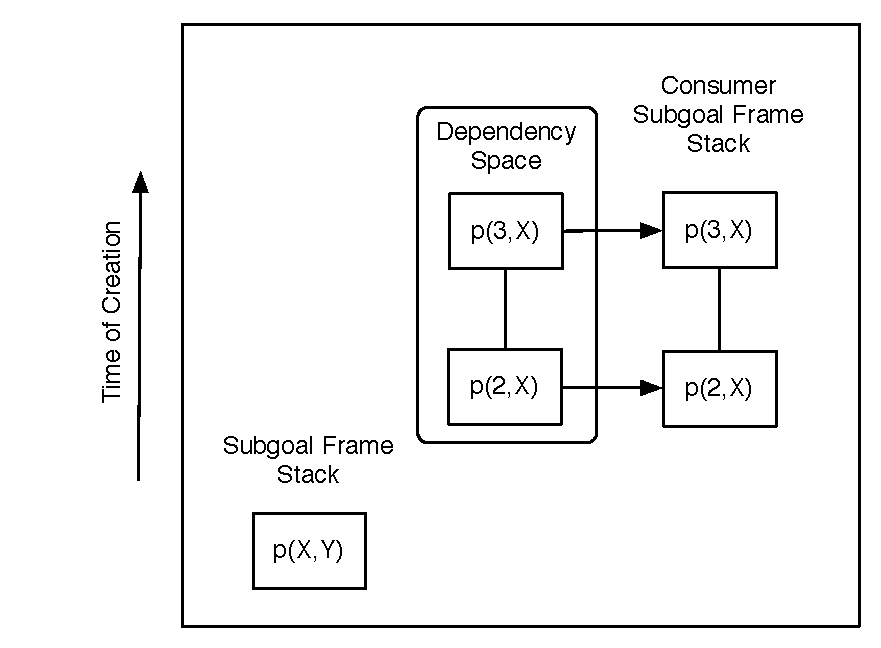
\includegraphics[scale=0.5]{completion_space.pdf}
  \caption{Subsumptive generator and consumers before completion.}
  \label{fig:completion_space}
\end{figure}

\subsection{Compiled Tries}

YapTab also implements the compiled tries optimization, but as described in Section \ref{sec:compiled_tries}
we needed to change each trie instruction to do unification instead of simple variable binding.

Another important modification was the hash instructions. Two new instructions were
implemented: \texttt{trie\_do\_hash} and \texttt{trie\_retry\_hash}.
The instruction \texttt{trie\_do\_hash} is executed once an hash table node is reached.
If the next term to unify is a variable (case 1) each hash bucket will be executed, if it is an instantiated term (case 2)
the indexed bucket will be executed first, followed by the variable bucket.

We use an hash choice point (\texttt{hash\_choice\_pt}) to execute each bucket.
For instantiated terms, the hash choice point is only allocated when both variable and indexed bucket
exist and are different. For variables, the choice point is always stored. The instruction
set to execute upon backtracking is \texttt{trie\_retry\_hash}.

An hash choice point is an WAM choice point extended with two new fields:
\textbf{last\_bucket} and \textbf{final\_bucket}.
The field \textbf{last\_bucket} points to the last executed bucket on case 1 or the
variable bucket for case 2.
The second field, \textbf{final\_bucket}, helps differentiate between
case 1 and 2, as in case 2 its value is NULL. In case 1 points to the final hash table bucket,
hence it is easy to know when to remove the choice point.

\section{Chapter Summary}

This chapter throughly explained the algorithms and data structures behind the Time Stamped Tries
technique to implement call by subsumption in a tabling engine. We discussed how the answer trie
was extended with time stamp information and explained the need for a time stamp index to efficiently
collect relevant answers for subsumed subgoals.

We discussed how the YapTab engine was extended with the Time Stamped Tries mechanisms to
provide tabling by call subsumption. We also showed how the core algorithms in YapTab were minimally
affected.

In the next chapter, we will present a new tabling extension called Retroactive Call Subsumption (RCS),
that improves upon call subsumption by enabling bidirectional sharing of answers, that is, answers will
be shared even if a subsumed subgoal is called before a subsuming subgoal.
